
\chapter{Maxima, minima and inflection points.}% Curve tracing.}


%79. 
\section{Introduction}
\label{sec:79}

A great many practical problems occur where we have to 
deal with functions of such a nature that they have a 
greatest (maximum) value or a least 
(minimum) value\footnote{There may be more than one of each.}
and it is very important to know what particular value of the 
variable gives such a value of the function. 

%{\small{
\begin{example}
\label{ex:circle}
{\rm
For instance, suppose that it is required to find the dimensions 
of the rectangle of greatest area that can be inscribed 
in a circle of radius $5$ inches. Consider the circle in 
Figure \ref{fig:circle-example}:

\begin{figure}[h!]
%\begin{tabular}{cc}
\begin{minipage}{\textwidth}
\begin{center}
%\vspace{1.0 cm}
%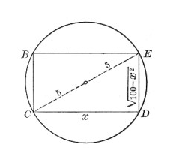
\includegraphics[height=4cm,width=4cm]{circle-example.eps}
\includegraphics[height=6cm,width=6cm]{circle-example3.eps}
\end{center}
\end{minipage}
%\caption{Scan of Granville's graphic of an inscribed circle with rectangle.}
\caption{A rectangle with circumscribed circle.}
\label{fig:circle-example}
\end{figure}
%sage: p1 = polar_plot(lambda x: 5, 0, 2*pi, rgbcolor=hue(0.6))
%sage: p2 = line([(-4,3),(4,3)])
%sage: p3 = line([(4,3),(4,-3)])
%sage: p4 = line([(-4,-3),(4,-3)])
%sage: p5 = line([(-4,-3),(-4,3)])
%sage: p6 = line([(-4,-3),(4,3)],linestyle="--")
%sage: t1 = text("$x$", (0.0,-3.2))
%sage: t2 = text("$\sqrt{100-x^2}$", (3.3,0.0))
%sage: t3 = text("B", (-4.3,3.0))
%sage: t4 = text("C", (-4.3,-3.0))
%sage: t5 = text("E", (4.3,3.0))
%sage: t6 = text("D", (4.3,-3.0))
%sage: t7 = text("$5$", (4.2/2-0.2,3.0/2+0.2))
%sage: d1 = disk((0.0,0.0), 0.07, (0, 2*pi), rgbcolor=(0,0,0))
%sage: show(p1+p2+p3+p4+p5+p6+t1+t2+t3+t4+t5+t6+t7+d1,axes=False)

\noindent
Inscribe any rectangle, as BCDE.
Let $CD = x$; then $DE = \sqrt{100 - x^2}$, and the area of the 
rectangle is evidently

\[
%(1) 
A = A(x) = x\sqrt{100 - x^2}.
\]
That a rectangle of maximum area must exist may be seen as follows: 
Let the base $CD$ ($= x$) increase to $10$ inches (the diameter); 
then the altitude $DE$ ($= \sqrt{100 - x^2}$) will decrease to zero 
and the area will become zero. Now let the base decrease to zero; 
then the altitude will increase to $10$ inches and the area will 
again become zero. It is therefore intuitionally evident that there 
exists a greatest rectangle. By a careful study of the figure 
we might suspect that when the rectangle becomes a square its 
area would be the greatest, but this would at best be mere 
guesswork. A better way would evidently be to plot the graph 
of the function $A=A(x)$ and note its behavior. To aid us in drawing 
the graph of $A(x)$, we observe that

\begin{itemize}
\item[(a)] from the nature of the problem it is 
evident that $x$ and $A$ must both be positive; and

\item[(b)] 
the values of $x$ range from zero to $10$ inclusive.
\end{itemize}
Now construct a table of values and draw the graph.
What do we learn from the graph?

\begin{figure}[h!]
%\begin{tabular}{cc}
\begin{minipage}{\textwidth}
\begin{center}
%\vspace{1.0 cm}
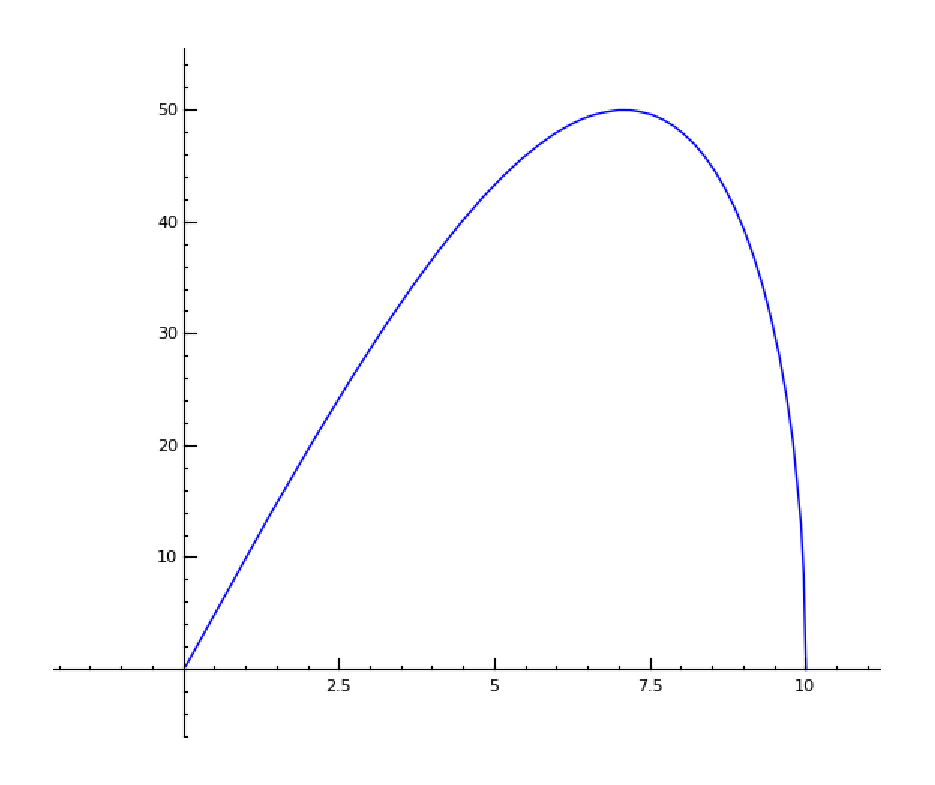
\includegraphics[height=4cm,width=7cm]{circle-example2.eps}
\end{center}
\end{minipage}
\caption{The area of a rectangle with fixed circumscribed circle.}
\label{fig:circle-example2}
\end{figure}
%sage: x = var("x")
%sage: P = plot(x*sqrt(100-x^2),0,1.11)
%sage: show(P)

(a) If the rectangle is carefully drawn, we may find quite accurately the area 
of the rectangle corresponding to any value $x$ by measuring 
the length of the corresponding ordinate. Thus,
when 	$x = OM = 3$ inches,
then 	$A = MP = 28.6$ square inches;
and when 	$x = ON = \frac{9}{2}$ inches,
then 	$A = NQ \approx 39.8$ sq. in. (found by measurement).

(b) There is one horizontal tangent (RS). The ordinate TH from its 
point of contact T is greater than any other ordinate. Hence this 
discovery: One of the inscribed rectangles has evidently a 
greater area than any of the others. In other words, we may 
infer from this that the function defined by $A=A(x)$ has a maximum 
value. We cannot find this value (= HT) exactly by measurement, 
but it is very easy to find, using Calculus methods. We 
observed that at T the tangent was horizontal; hence the 
slope will be zero at that point (Example \ref{ex:64}). %1, p. 74 [§64]). 
To find the abscissa of T we then find the first 
derivative of $A(x)$, place it equal to zero, and solve for $x$. Thus

\[
%(1) 	
\begin{array}{ll}
\ A 	&= x\sqrt{100 - x^2},\\
  \frac{dA}{dx} &=\ \frac{100 - 2 x^2}{\sqrt{100 - x^2}},\\
  \frac{100 - 2 x^2}{\sqrt{100 - x^2}} 	&=\ 0.
\end{array}
\]
Solving, $ x 	=\ 5\sqrt{2}$.
Substituting back, we get $ DE 	= \sqrt{100 - x^2} = 5\sqrt{2}$.
Hence the rectangle of maximum area inscribed in the circle is 
a square of area
$A = CD \times DE = 5\sqrt{2} \times 5\sqrt{2} = 50$ square inches. 
The length of HT is therefore $50$.

}
\end{example}
%}}


\begin{example}
\label{ex:box}
{\rm
A wooden box is to be built to contain $108$ cu. ft. It 
is to have an open top and a square base. What must be its 
dimensions in order that the amount of material required 
shall be a minimum; that is, what dimensions will make the 
cost the least?

\begin{figure}[h!]
%\begin{tabular}{cc}
\begin{minipage}{\textwidth}
\begin{center}
%\vspace{1.0 cm}
%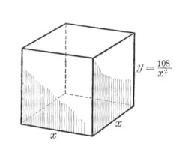
\includegraphics[height=3cm,width=3cm]{volume-box.eps}
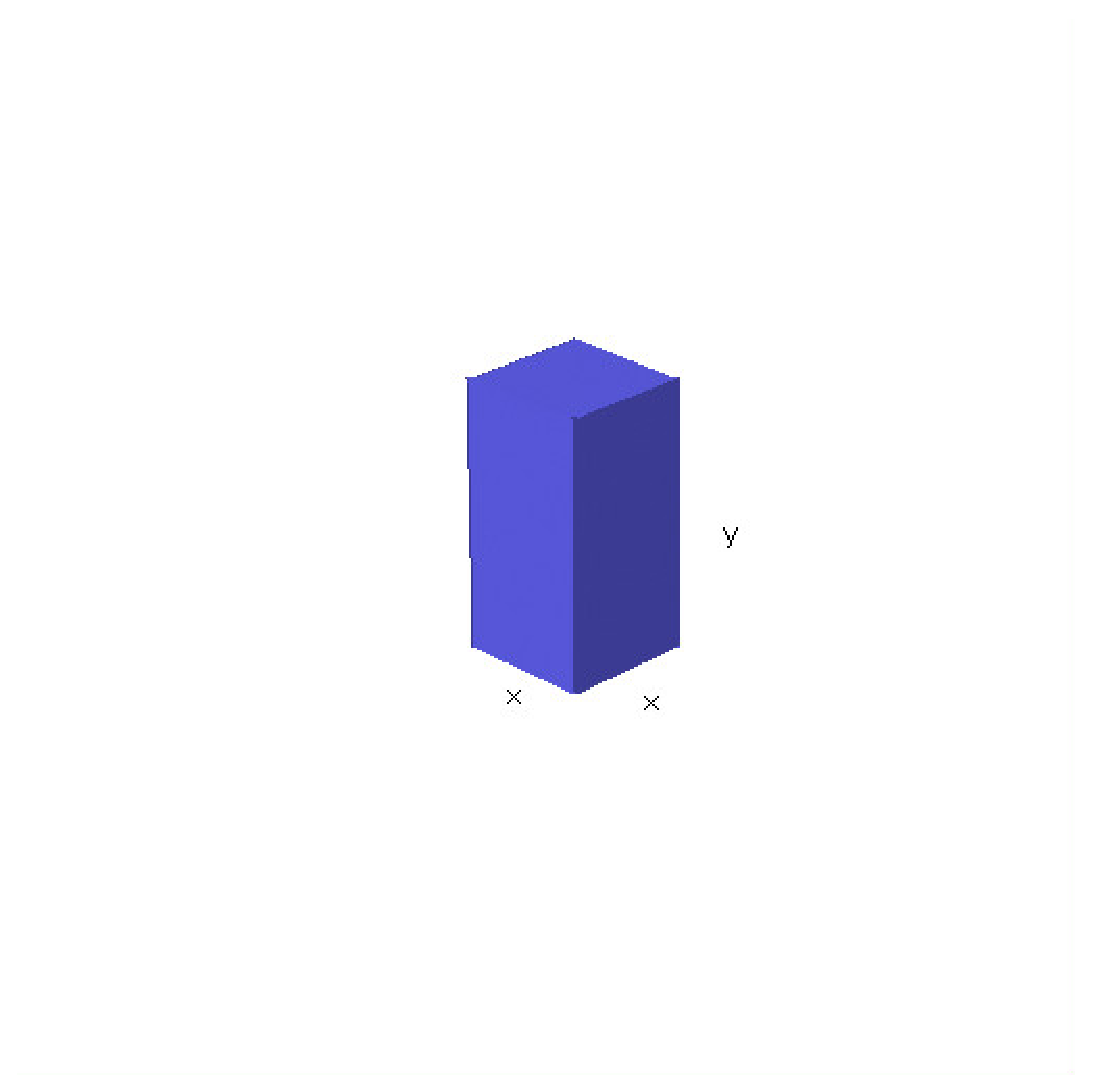
\includegraphics[height=6cm,width=5cm]{volume-box3b.eps}
\end{center}
\end{minipage}
\caption{A box with square $x\times x$ base, height $y=108/x^2$, 
and fixed volume.}
%\caption{Scan of Granville's graphic of a box with square base and fixed volume.}
\label{fig:volume-box}
\end{figure}
%sage: p1 = cube(aspect_ratio=[1,1,1]).scale([1,1,2])
%sage: from sage.plot.plot3d.shapes2 import text3d
%sage: p2 = text3d("y",(1,1/2,0))
%sage: p3 = text3d("x",(1,-1/4,-1))
%sage: p4 = text3d("x",(1,-3/2,-0.5))
%sage: (p1+p2+p3+p4).show(frame=False)


\noindent
Let $x$ denote the length of side of square base in feet,
and $y$ denote the height of box.
Since the volume of the box is given, $y$ may be found in terms of $x$. Thus
${\rm volume} =\ x^2 y\ =\ 108$,
so $y\ =\ \frac{108}{x^2}$.
We may now express the number (= $M$) of square feet of lumber required 
as a function of $x$ as follows: 

\begin{center}
area of base = 	$x^2$ sq. ft.,
\\
area of four sides = $4xy\ =\ \frac{432}{x}$ sq. ft. 
\end{center}
Hence

\[
%(2)
M = M(x)	=\ x^2 + \frac{432}{x}
\]
is a formula giving the number of square feet required in 
any such box having a capacity of $108$ cu. ft. 
Draw a graph of $M(x)$.

\begin{figure}[h!]
%\begin{tabular}{cc}
\begin{minipage}{\textwidth}
\begin{center}
%\vspace{1.0 cm}
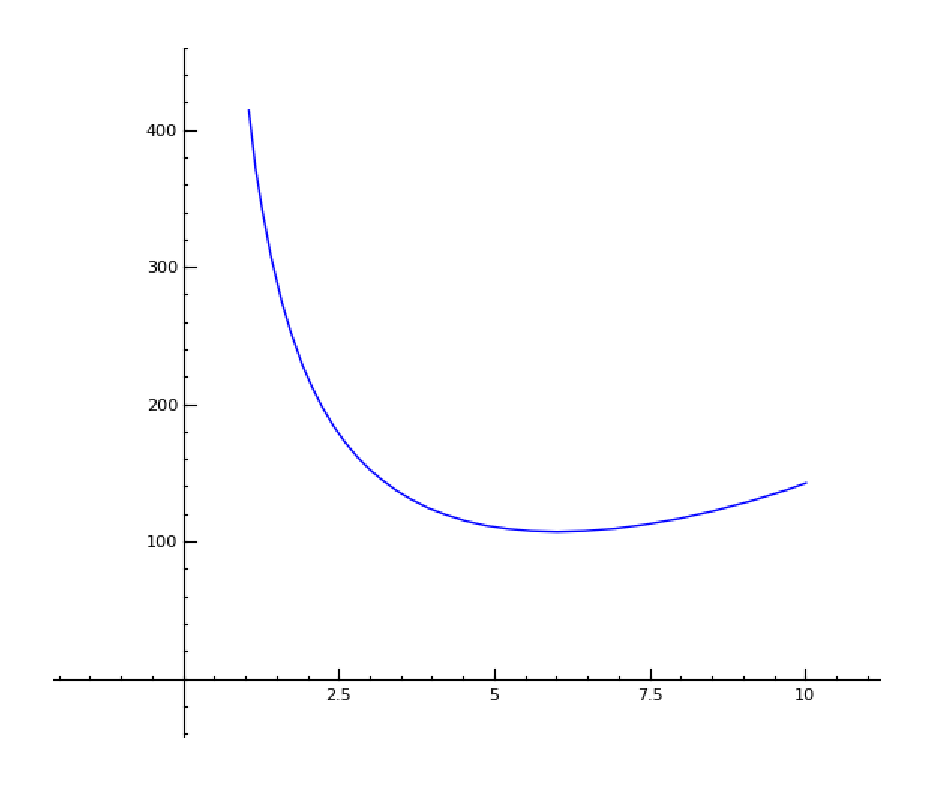
\includegraphics[height=4cm,width=7cm]{volume-box2.eps}
\end{center}
\end{minipage}
\caption{\sage plot of $y=x^2 + \frac{432}{x}$, $1<x<10$.}
\label{fig:volume-box2}
\end{figure}
%sage: P = plot(x^2 + 432/x,1,10)
%sage: show(P)

What do we learn from the graph?

(a) If the box is carefully drawn, we may measure the ordinate corresponding 
to any length ($= x$) of the side of the square base and so determine 
the number of square feet of lumber required.

(b) There is one horizontal tangent (RS). The ordinate from its 
point of contact T is less than any other ordinate. 
Hence this discovery: One of the boxes evidently takes less lumber 
than any of the others. In other words, we may infer that the 
function defined by $M=M(x)$ has a minimum value. Let us find this 
point on the graph exactly, using our Calculus. Differentiating $M(x)$
to get the slope at any point, we have

\[
    \frac{dM}{dx} = 2x - \frac{432}{x^2}.
\]
At the lowest point T the slope will be zero. Hence

\[
  2x - \frac{432}{x^2} = 0;
\]
that is, when $x = 6$ the least amount of lumber will be needed.

Substituting in $M(x)$, we see that this is $M = 108$ sq. ft.

The fact that a least value of $M$ exists is also shown by the 
following reasoning. Let the base increase from a very small square to 
a very large one. In the former case the height must be very great 
and therefore the amount of lumber required will be large. In the 
latter case, while the height is small, the base will take a 
great deal of lumber. Hence $M$ varies from a large value, grows less, 
then increases again to another large value. It follows, then, 
that the graph must have a ``lowest'' point corresponding to the 
dimensions which require the least amount of lumber, and therefore 
would involve the least cost.

Here is how to compute the critical points in \sage:

\vskip .1in

\begin{Verbatim}[fontsize=\small,fontfamily=courier,fontshape=tt,frame=single,label=\sage]

sage: x = var("x")
sage: f = x^2 + 432/x
sage: solve(f.diff(x)==0,x)
[x == 3*sqrt(3)*I - 3, x == -3*sqrt(3)*I - 3, x == 6]

\end{Verbatim}
\vskip .1in

\noindent
This says that $(x^2 + 432/x)'=0$ has three roots, but only one
real root - the one reported above at $x=6$.
}
\end{example}

We will now proceed to the treatment in detail of the subject 
of maxima and minima.

%80. 
\section{Increasing and decreasing functions}
\footnote{The proofs given here depend chiefly on geometric 
intuition.}
%The subject of Maxima and Minima will be treated 
%analytically in \ref{sec:108}.} %§108, p. 167.

A function is said to be {\it increasing} when it increases as 
the variable increases and decreases as the variable decreases. 
A function is said to be {\it decreasing} when it decreases 
as the variable increases and increases as the variable decreases.
\index{function! increasing}
\index{function! decreasing}

The graph of a function indicates plainly whether it is 
increasing or decreasing. 

\begin{example}
{\rm
(1) For instance, consider the function $a^x$ whose graph 
(Figure \ref{fig:exp-fcn2}) is the locus of the equation
$y = a^x$, $a > 1$:

\begin{figure}[h!]
%\begin{tabular}{cc}
\begin{minipage}{\textwidth}
\begin{center}
%\vspace{1.0 cm}
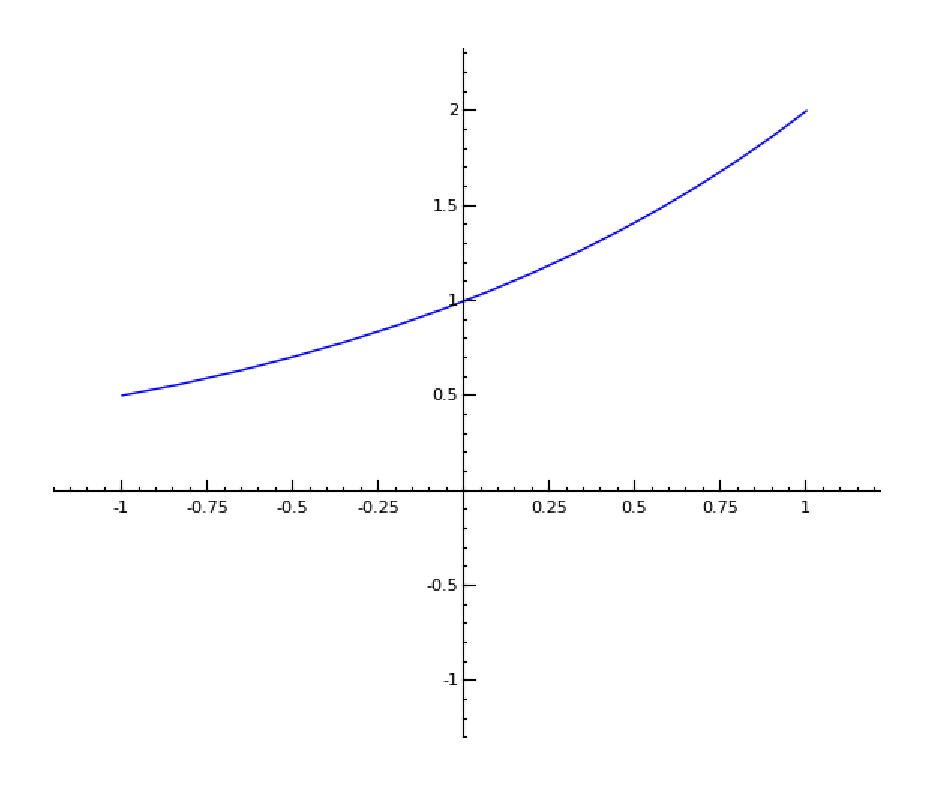
\includegraphics[height=4cm,width=4cm]{exp-fcn2.eps}
\end{center}
\end{minipage}
\caption{\sage plot of $y=2^x$, $-1<x<1$.}
\label{fig:exp-fcn2}
\end{figure}
%sage: P = plot(e^(ln(2)*x),-1,1)
%sage: show(P)

As we move along the curve from left to right the curve is rising; 
that is, as $x$ increases the function ($= y$) always increases. Therefore 
$a^x$ is an increasing function for all values of $x$.

(2) On the other hand, consider the function $(a - x)^3$ whose graph 
(Figure \ref{fig:cubic-fcn2}) is the locus of the equation $y = (a - x)^3$.

\begin{figure}[h!]
%\begin{tabular}{cc}
\begin{minipage}{\textwidth}
\begin{center}
%\vspace{1.0 cm}
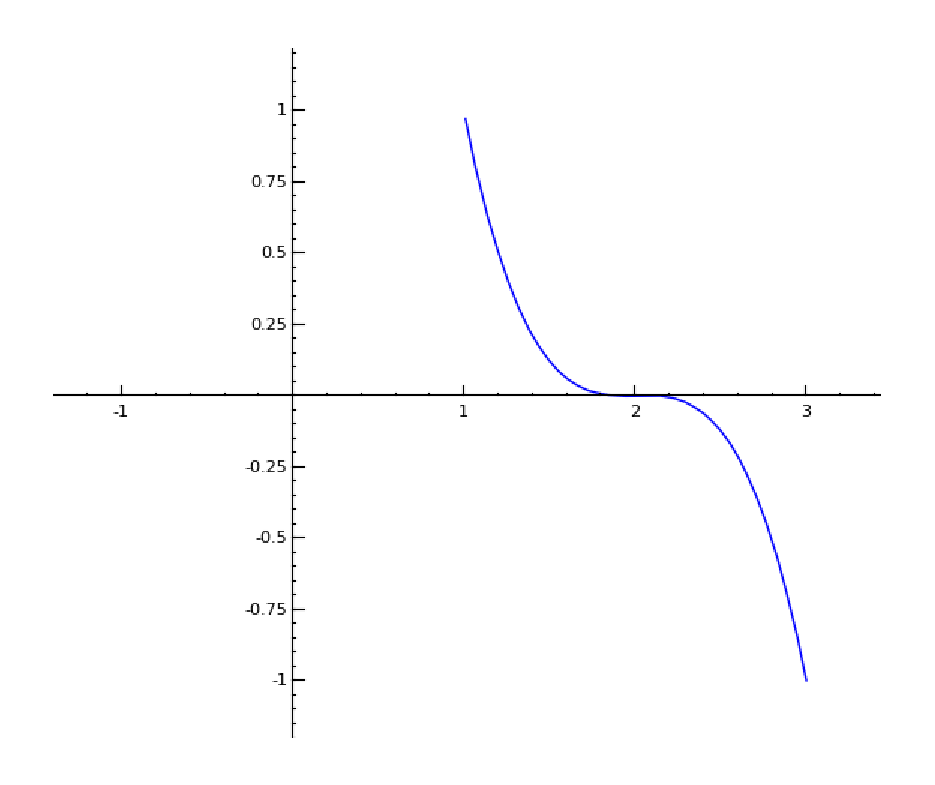
\includegraphics[height=4cm,width=7cm]{cubic-fcn2.eps}
\end{center}
\end{minipage}
\caption{\sage plot of $y=(2-x)^3$, $1<x<3$.}
\label{fig:cubic-fcn2}
\end{figure}
%sage: P = plot((2-x)^3,1,3)
%sage: show(P)

\noindent
Now as we move along the curve from left to right the curve is 
falling; that is, as $x$ increases, the function ($= y$) always 
decreases. Hence $(a - x)^3$ is a decreasing function for all values of $x$.

(3) That a function may be sometimes increasing and sometimes 
decreasing is shown by the graph (Figure \ref{fig:cubic-fcn3}) of

\[
    y = 2x^3 - 9x^2 + 12x - 3.
\]

\begin{figure}[h!]
%\begin{tabular}{cc}
\begin{minipage}{\textwidth}
\begin{center}
%\vspace{1.0 cm}
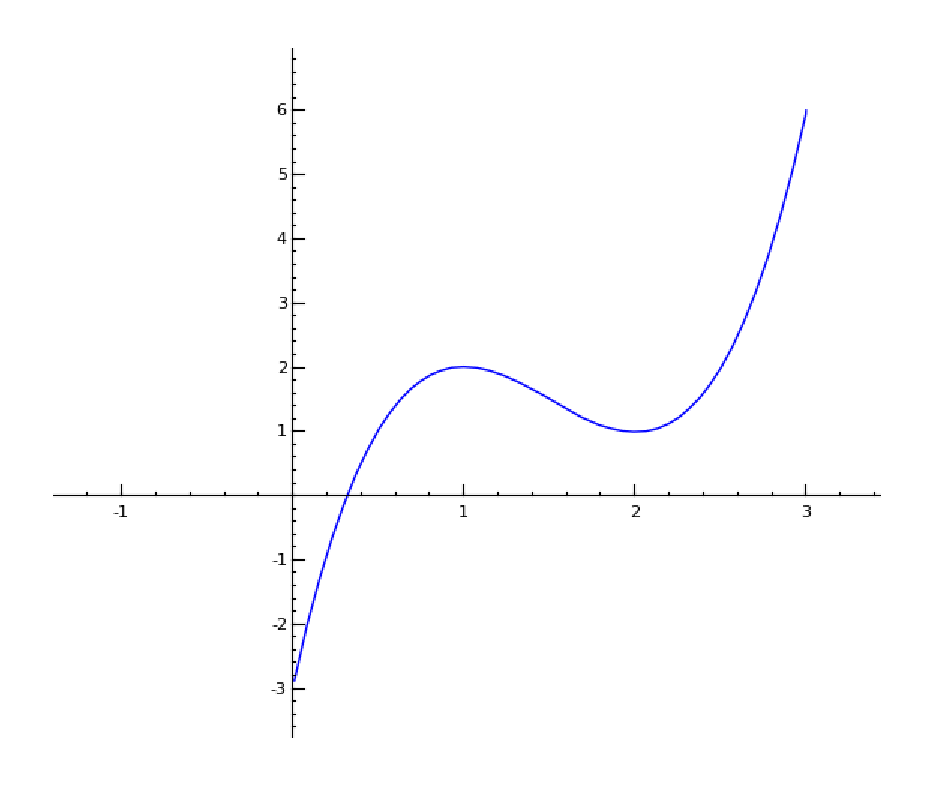
\includegraphics[height=4cm,width=7cm]{cubic-fcn3.eps}
\end{center}
\end{minipage}
\caption{\sage plot of $y=2x^3 - 9x^2 + 12x - 3$, $0<x<3$.}
\label{fig:cubic-fcn3}
\end{figure}
%sage: P = plot(2*x^3 - 9*x^2 + 12*x - 3,0,3)
%sage: show(P)


As we move along the curve from left to right the curve rises 
until we reach the point A when $x=1$, then it falls from A to the point B
when $x=2$, and to the  right of B it is always rising. Hence

\begin{itemize}
\item[(a)] from $x = -\infty$ to $x = 1$ the function is increasing;

\item[(b)] from $x = 1$ to $x = 2$ the function is decreasing;

\item[(c)] from $x = 2$ to $x = +\infty$ the function is increasing.
\end{itemize}

The student should study the curve carefully in order to note 
the behavior of the function when $x = 1$ and $x = 2$. Evidently A and B 
are turning points. At A the function ceases to increase and 
commences to decrease; at B, the reverse is true. At A and B the 
tangent (or curve) is evidently parallel to the $x$-axis, and 
therefore the slope is zero.
}
\end{example}

%81. 
\section{Tests for determining when a function is increasing or decreasing}
\label{sec:81}

It is evident from Figure \ref{fig:cubic-fcn3} that at a point where a function

\[
    y = f(x)
\]
is increasing, the tangent in general makes an acute angle with the 
$x$-axis; hence

\begin{center}
    slope $= \tan\, \tau = \frac{dy}{dx} = f'(x) =$ a positive number.
\end{center}
Similarly, at a point where a function is decreasing, the 
tangent in general makes an obtuse angle with the $x$-axis; 
therefore\footnote{Conversely, for any given value of $x$, if 
$f'(x) >0$, then $f(x)$ is increasing; if $f'(x) < 0$, then 
$f(x)$ is decreasing. When $f'(x) = 0$, we cannot decide without 
further investigation whether $f(x)$ is increasing or decreasing.}

\begin{center}
    slope $= \tan\, \tau = \frac{dy}{dx} = f'(x) =$ a negative number.
\end{center}
In order, then, that the function shall change from an increasing 
to a decreasing function, or vice versa, it is a necessary and 
sufficient condition that the first derivative shall change 
sign. But this can only happen for a continuous derivative by 
passing through the value zero. Thus in Figure \ref{fig:cubic-fcn3}
as we pass along the curve the derivative (= slope) changes sign 
at the points where $x=1$ and $x=2$. In general, then, we 
have at ``turning points,''
\index{turning points}

\[
%(18) 
\frac{dy}{dx} = f'(x) = 0. 
\]
A value of $y=f(x)$ satisfying this condition is called a 
{\it critical point} of the function $f(x)$. %% new
\index{critical point}
The derivative is continuous in nearly all our important 
applications, but it is interesting to note the case when the derivative 
(= slope) changes sign by passing through\footnote{By this is meant 
that its reciprocal passes through the value zero.} $\infty$. 
This would evidently happen at the points one a curve where the 
tangents (and curve) are perpendicular to the $x$-axis. At such 
exceptional critical points %turning points

\[
    \frac{dy}{dx} = f'(x) = \inf;
\]
or, what amounts to the same thing,

\[
    \frac{1}{f'(x)} = 0.
\]

%82. 
\section{Maximum and minimum values of a function}
\label{sec:82}

A {\it maximum value} of a function is one that is greater 
than any values immediately preceding or following.
A {\it minimum value} of a function is one that is less than 
any values immediately preceding or following.
\index{maximum value}
\index{minimum value}

For example, in Figure \ref{fig:cubic-fcn3}, it is clear that the 
function has a maximum value ($y = 2$) when $x = 1$, and a 
minimum value ($y = l$) when $x = 2$.

The student should observe that a maximum value is not 
necessarily the greatest possible value of a function nor a 
minimum value the least. For in Figure \ref{fig:cubic-fcn3} it is seen that 
the function ($= y$) has values to the right of $x=1$ that are 
greater than the maximum $2$, and values to the left of $x=1$ that 
are less than the minimum $1$.

\begin{figure}[h!]
%\begin{tabular}{cc}
\begin{minipage}{\textwidth}
\begin{center}
%\vspace{1.0 cm}
%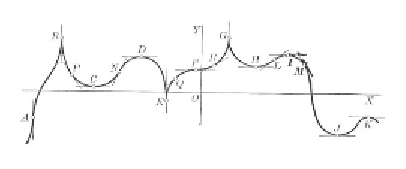
\includegraphics[height=3cm,width=6cm]{crazy-fcn.eps}
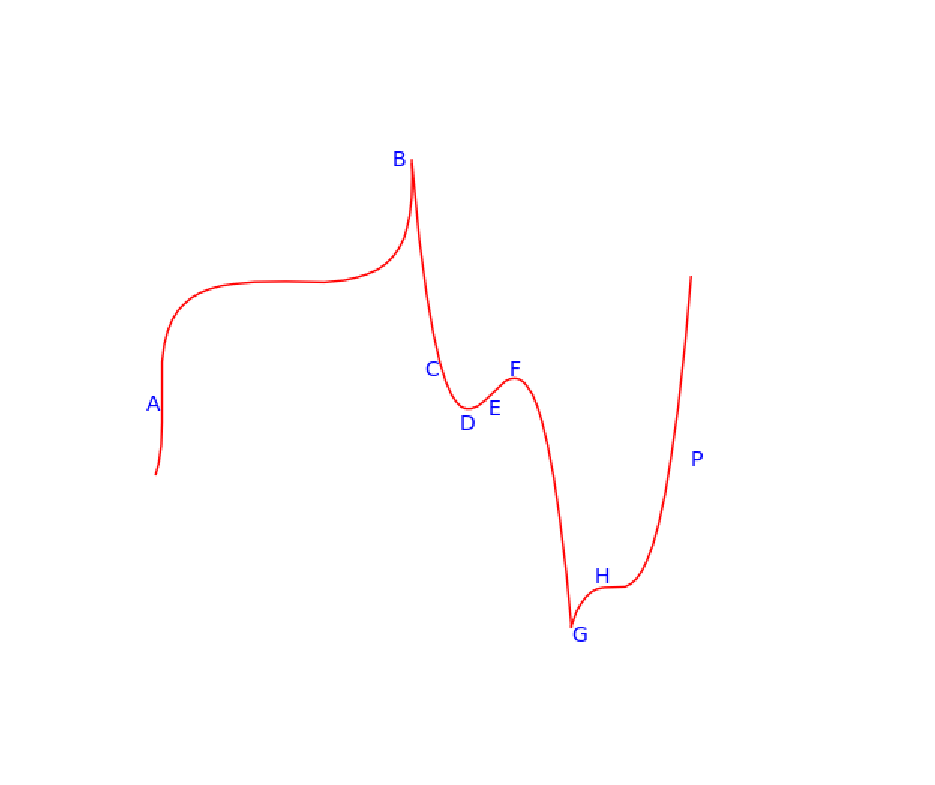
\includegraphics[height=7cm,width=11cm]{curve-tangent3.eps}
\end{center}
\end{minipage}
%\caption{Scan of Granville's graphic of a continuous function.}
\caption{A continuous function.}
\label{fig:crazy-fcn}
\end{figure}
%sage: t = var("t")
%sage: f1 = lambda t: [t-sin(t),sin(t)+t]
%sage: p1 = parametric_plot(f1(t), -1, 2*pi, rgbcolor=(1,0,0))
%sage: f2 = lambda t: [t + 2 + 2*RR(pi), 1 + t - t^3 - 7 + 2*RR(pi)]
%sage: p2 = parametric_plot( f2(t), -2, 2, rgbcolor=(1,0,0))
%sage: f3 = lambda t: [t+5+2*RR(pi), t^3-11+2*RR(pi)]
%sage: p3 = parametric_plot( f3(t), -1, 2, rgbcolor=(1,0,0))
%sage: t1 = text('A', (-0.2, 0.0))
%sage: t2 = text('B', (6.0, 6.3))
%sage: t3 = text('C', (6.8, 0.9))
%sage: t4 = text('D', (7.7, -0.5))
%sage: t5 = text('E', (8.4, -0.1))
%sage: t6 = text('F', (8.9, 0.9))
%sage: t7 = text('G', (f3(-1)[0]+0.2, f3(-1)[1]-0.2))
%sage: t8 = text('H', (f3(-1)[0]+0.8, f3(-1)[1]+1.3))
%sage: t9 = text('P', (f3(-1)[0]+3.2, f3(-1)[1]+4.3))
%sage: show(p1+p2+p3+t1+t2+t3+t4+t5+t6+t7+t8+t9)
%sage: show(p1+p2+p3+t1+t2+t3+t4+t5+t6+t7+t8+t9,axes=False)

A function may have several maximum and minimum values. Suppose 
that Figure \ref{fig:crazy-fcn} represents the graph of a function $f(x)$.

At B, F the function is at a local maximum, and at D, G 
a minimum. That some particular minimum value of a function 
may be greater than some particular maximum value is 
shown in the figure, the minimum value at D being greater 
than the maximum value at G.

At the ordinary critical %turning 
points D, F, H the tangent (or curve) is parallel to the $x$-axis; 
therefore

\[
{\rm   slope} = \frac{dy}{dx} = f'(x) = 0.
\]
At the exceptional critical %turning 
points A, B, G the tangent (or curve) is perpendicular to the $x$-axis, 
giving

\[
{\rm  slope} = \frac{dy}{dx} = f'(x) = \infty . 
\]

One of these two conditions is then necessary in order that 
the function shall have a maximum or a minimum value. But such 
a condition is not sufficient; for at H the slope is zero and 
at A it is infinite, and yet the function has neither a maximum nor a 
minimum value at either point. It is necessary for us to know, in 
addition, how the function behaves in the neighborhood of each point. 
Thus at the points of maximum value, B, F, the function 
changes from an increasing to a decreasing function, and at the 
points of minimum value, D, G, the function changes from a 
decreasing to an increasing function. It therefore follows from 
\S \ref{sec:81} %§ 81 
that at maximum points

\begin{center}
    slope $= \frac{dy}{dx} = f'(x)$ must change from + to -,
\end{center}
and at minimum points

\begin{center}
    slope $= \frac{dy}{dx} = f'(x)$ must change from - to +
\end{center}
when we move along the curve from left to right.

At such points as A and H where the slope is zero or infinite, 
but which are neither maximum nor minimum points,

\begin{center}
    slope $= \frac{dy}{dx} = f'(x)$ does not change sign.
\end{center}
We may then state the conditions in general for maximum and minimum 
values of $f(x)$ for certain values of the variable as follows:

\begin{equation}
%(19) 
f(x) \ {\rm is\ a\ maximum\ if\ }f'(x) = 0, \ {\rm and}\ f'(x)\
{\rm changes\ from\ } +\ {\rm to}\ -.
\label{eqn:19-82}
\end{equation}

\begin{equation}
%(20) 
f(x)  \ {\rm is\ a\ minimum\ if}\ f'(x) = 0,\ {\rm and}\ f'(x)\ 
{\rm changes\ from}\ -\ {\rm to}\ +.
\label{eqn:20-82}
\end{equation}

The values of the variable at the turning points of a function 
are called {\it critical values}; thus $x = 1$ and $x = 2$ are the 
critical values of the variable for the function whose 
graph is shown in Figure \ref{fig:cubic-fcn3}. %Fig. c, p. 107. 
The critical values at turning points where the 
tangent is parallel to the $x$-axis are evidently found by 
placing the first derivative equal to zero and solving 
for real values of $x$, just as under \S \ref{sec:64}. %§ 64, p. 73.
\index{critical value}
(Similarly, if we wish to examine a function at exceptional 
turning points where the tangent is perpendicular to the $x$-axis, 
we set the reciprocal of the first derivative equal to 
zero and solve to find critical values.)

To determine the sign of the first derivative at points near 
a particular turning point, substitute in it, first, a value 
of the variable just a little less than the corresponding critical 
value, and then one a little greater\footnote{In this connection the 
term ``little less,'' or ``trifle less,'' means any value between 
the next smaller root (critical value) and the one under 
consideration; and the term ``little greater,'' or ``trifle greater,''
means any value between the root under consideration and the next larger one.}. 
If the first gives $+$ (as at L, Figure \ref{fig:crazy-fcn}) 
% Fig. d, p. 109 [§82]) 
and the second - (as at M), then the function ($= y$) has a maximum value 
in that interval (as at I).
If the first gives $-$ (as at P) and the second $+$ (as at N), then 
the function ($= y$) has a minimum value in that interval (as at C).

If the sign is the same in both cases (as at Q and R), 
then the function ($= y$) has neither a maximum nor a minimum 
value in that interval (as at F)\footnote{A similar discussion 
will evidently hold for the exceptional turning points B, E, and A 
respectively.}.

We shall now summarize our results into a compact working rule.


%83. 
\section{Examining a function for extremal values: first method}
%maximum and minimum values.}

Working rule:

\begin{itemize}
\item
FIRST STEP. Find the first derivative of the function.

\item
SECOND STEP. Set the first derivative equal to 
zero\footnote{When the first derivative becomes infinite for a 
certain value of the independent variable, then the function 
should be examined for such a critical value of the variable, for 
it may give maximum or minimum values, as at B, E, or A 
(Figure \ref{fig:crazy-fcn}). %Fig. d, p. 109). 
See footnote in \S \ref{sec:81}.} %p. 108 [§81].}
and solve the resulting equation for real roots in order to 
find the critical values of the variable.

\item
THIRD STEP. Write the derivative in factor form; if it is algebraic, 
write it in linear form.

\item
FOURTH STEP. Considering one critical value at a time, test the first 
derivative, first for a value a trifle less and then for a value a 
trifle greater than the critical value. If the sign of the 
derivative is first $+$ and then $-$, the function has a maximum value 
for that particular critical value of the variable; but if the 
reverse is true, then it has a minimum value. If the sign does 
not change, the function has neither.
\end{itemize}

\begin{example}
{\rm
In the problem worked out in Example \ref{ex:circle}, %on p. 104 [§79] 
we showed by means of the graph of the function

\[
    A = x\sqrt{100 - x^2}
\]
that the rectangle of maximum area inscribed in a circle 
of radius $5$ inches contained $50$ square inches. This may now 
be proved analytically as follows by applying the above rule.

Solution. $f(x)=x\sqrt{100 - x^2}$.

First step. $f'(x) 	=\ \frac{100 - 2x^2}{\sqrt{100 - x^2}}$.

Second step. $\frac{100 - 2x^2}{\sqrt{100 - x^2}} 	=\ 0$
implies $ x 	=\ 5\sqrt{2}$, which is the critical value. Only 
the positive sign of the radical is taken, since, from the 
nature of the problem, the negative sign has no meaning.

Third step. $ f'(x) 
=\ \frac{2(5\sqrt{2} - x)(5\sqrt{2} + x)}{\sqrt{(10 - x)(10 + x)}}$.

Fourth step. When $x < 5\sqrt{2}$, $f'(x) 	=\ \frac{2(+)(+)}{\sqrt{(+)(+)}} = +$.
When $x > 5\sqrt{2}$, $f'(x) 	=\ \frac{2(+)(+)}{\sqrt{(-)(+)}} = -$.

Since the sign of the first derivative changes from $+$ to $-$ 
at $x = 5\sqrt{2}$, the function has a maximum value

\[
    f(5\sqrt{2}) = 5\sqrt{2} \cdot 5\sqrt{2} = 50. 
\]

In \sage:

\vskip .1in

\begin{Verbatim}[fontsize=\small,fontfamily=courier,fontshape=tt,frame=single,label=\sage]

sage: x = var("x")
sage: f(x) = x*sqrt(100 - x^2)
sage: f1(x) = diff(f(x),x); f1(x)
sqrt(100 - x^2) - x^2/sqrt(100 - x^2)
sage: crit_pts = solve(f1(x) == 0,x); crit_pts
[x == -5*sqrt(2), x == 5*sqrt(2)]
sage: x0 = crit_pts[1].rhs(); x0
5*sqrt(2)
sage: f(x0)
50
sage: RR(f1(x0-0.1))>0
True
sage: RR(f1(x0+0.1))<0
True

\end{Verbatim}
\vskip .1in
\noindent
This tells us  that $x_0=5\sqrt{2}$ is a critical point, at
which the area is $50$ square inches and at which the
area changes from increasing to decreasing. This implies that the
area is a maximum at this point.

}
\end{example}

%84. 
\section{Examining a function for extremal values: second method} 
\label{sec:84}

From (\ref{eqn:19-82}), %p. 110 [§82], 
it is clear that in the vicinity of a maximum value of $f(x)$, in 
passing along the graph from left to right,
$f'(x)$ changes from $+$ to $0$ to $-$.
Hence $f'(x)$ is a decreasing function, and by \S \ref{sec:81} %§81 
we know that its derivative, i.e. the second derivative ($= f''(x)$)
of the function itself, is negative or zero.

Similarly, we have, from (\ref{eqn:20-82}), %p. 110, 
that in the vicinity of a minimum value of $f(x)$
$f'(x)$ changes from $-$ to $0$ to $+$.
Hence $f'(x)$ is an increasing function and by \S \ref{sec:81} %§81 
it follows that $f''(x)$ is positive or zero.

The student should observe that $f''(x)$ is positive not only 
at minimum values but also at ``nearby'' points, $P$ say, to
the right of such a critical point. For, as a point 
passes through P in moving from left to right,
slope $= \tan \tau = \frac{dy}{dx} = f'(x)$ is an increasing function.
At such a point the curve is said to be {\it concave upwards}.
\index{concave upward}
Similarly, $f''(x)$ is negative not only at maximum points 
but also at ``nearby ''points, $Q$ say, to the left of such
a critical point. For, as a point passes through $Q$,
slope $= \tan \tau = \frac{dy}{dx} = f'(x)$ is a decreasing function.
At such a point the curve is said to be {\it concave downwards}.

At a point where the curve is concave upwards we sometimes say that 
the curve has a ``positive bending,]] and where it is concave 
downwards a ``negative bending.''

We may then state the sufficient conditions for maximum and minimum 
values of $f(x)$ for certain values of the variable as follows:

\begin{equation}
%(21) 
f(x)\ {\rm is\ a\ maximum\ if\ }f'(x) = 0\ {\rm and}\ f''(x) 
=\ {\rm a\ negative\ number}.
\label{eqn:84-21}
\end{equation}

\begin{equation}
%(22) 
f(x)\ {\rm is\ a\ minimum\ if}\ f'(x) = 0\ {\rm and}\ f''(x) 
=\ {\rm a\ positive\ number}.
\label{eqn:84-22}
\end{equation}
Following is the corresponding working rule.

\begin{itemize}
\item
FIRST STEP. Find the first derivative of the function.

\item
SECOND STEP. Set the first derivative equal to zero and 
solve the resulting equation for real roots in order to find 
the critical values of the variable.

\item
THIRD STEP. Find the second derivative.

\item
FOURTH STEP. Substitute each critical value for the variable in 
the second derivative. If the result is negative, then the 
function is a maximum for that critical value; if the result 
is positive, the function is a minimum.

\end{itemize}

When $f''(x) = 0$, or does not exist, the above process fails, 
although there may even then be a maximum or a minimum; in 
that case the first method given in the last section still 
holds, being fundamental. Usually this second method does 
apply, and when the process of finding the second derivative 
is not too long or tedious, it is generally the shortest method.

\begin{example}
{\rm
Let us now apply the above rule to test analytically the function

\[
   M = x^2 + \frac{432}{x}
\]
found in Example \ref{ex:box}. %the example worked out on p. 105 [§79].

Solution. $f(x) =\ x^2 + \frac{432}{x}$.

First step. $f'(x) 	=\ 2x - \frac{432}{x^2}$.

Second step. $2x - \frac{432}{x^2} 	=\ 0$.

Third step. $f''(x) 	=\ 2 + \frac{864}{x^3}$.

Fourth step. $f''(6) 	=\ +$. Hence $f(6) = 108$, 
minimum value.

In \sage:

\vskip .1in

\begin{Verbatim}[fontsize=\small,fontfamily=courier,fontshape=tt,frame=single,label=\sage]


sage: x = var("x")
sage: f(x) = x^2 + 432/x
sage: f1(x) = diff(f(x),x); f1(x)
2*x - 432/x^2
sage: f2(x) = diff(f(x),x,2); f2(x)
864/x^3 + 2
sage: crit_pts = solve(f1(x) == 0,x); crit_pts
[x == 3*sqrt(3)*I - 3, x == -3*sqrt(3)*I - 3, x == 6]
sage: x0 = crit_pts[2].rhs(); x0
6
sage: f2(x0)
6
sage: f(x0)
108

\end{Verbatim}
\vskip .1in
\noindent
This tells us that $x_0=6$ is a critical point and that $f''(x_0)>0$,
so it is a minimum.

}
\end{example}

The work of finding maximum and minimum values may 
frequently be simplified by the aid of the following 
principles, which follow at once from our discussion of the subject.

\begin{itemize}
\item[(a)] 
The maximum and minimum values of a continuous function must occur alternately,

\item[(b)] 
When $c$ is a positive constant, $c \cdot f(x)$ is a maximum 
or a minimum for such values of $x$, and such only, as make $f(x)$ 
a maximum or a minimum.

Hence, in determining the critical values of x and testing for maxima and 
minima, any constant factor may be omitted.

When $c$ is negative, $c \cdot f(x)$ is a maximum when $f(x)$ is 
a minimum, and conversely.

\item[(c)] 
If $c$ is a constant, $f(x)$ and $c + f(x)$
have maximum and minimum values for the same values of $x$.

Hence a constant term may be omitted when finding critical values of 
$x$ and testing.
\end{itemize}

In general we must first construct, from the conditions given in 
the problem, the function whose maximum and minimum values are 
required, as was done in the two examples worked out 
in \S \ref{sec:79}. %on pp. 103-106 [§79]. 
This is sometimes a problem of considerable difficulty. No rule 
applicable in all cases can be given for constructing the 
function, but in a large number of problems we may be guided by the following

General directions.

\begin{itemize}
\item[(a)] 
Express the function whose maximum or minimum is involved in the problem.

\item[(b)] 
If the resulting expression contains more than only variable, 
the conditions of the problem will furnish enough relations 
between the variables so that all may be expressed in terms of a single one.

\item[(c)] 
To the resulting function of a single variable apply one of 
our two rules for finding maximum and minimum values.

\item[(d)] 
In practical problems it is usually easy to tell which 
critical value will give a maximum and which a minimum value, 
so it is not always necessary to apply the fourth step of our rules.

\item[(e)] 
Draw the graph of the function in order to check the work.

\end{itemize}

\section{Problems}

\begin{enumerate}

\item
%1
It is desired to make an open-top box of greatest possible volume 
from a square piece of tin whose side is a, by cutting equal 
squares out of the corners and then folding up the tin to form the 
sides. What should be the length of a side of the squares cut out?

Solution. Let 	$x$ 	= side of small square = depth of box;
then 	$a - 2x$ 	= side of square forming bottom of box,
and volume is 	$V 	= (a - 2x)^2x$,
which is the function to be made a maximum by varying $x$. Applying rule:

First step. $\frac{dV}{dx} = (a - 2x)^2 - 4x(a - 2x) = a^2 - 8ax + 12x^2$.

Second step. Solving $a^2 - 8ax + 12x^2 = 0$ gives critical values 
$x = \frac{a}{2}$ and $\frac{a}{6}$.

It is evident that $x = \frac{a}{2}$ must give a minimum, for 
then all the tin would be cut away, leaving no material out of 
which to make a box. By the usual test, $x = \frac{a}{6}$ is found 
to give a maximum volume $\frac{2a^3}{27}$. Hence the side of the 
square to be cut out is one sixth of the side of the given square.

The drawing of the graph of the function in this 
and the following problems is left to the student.

\item
%2
Assuming that the strength of a beam with rectangular cross section 
varies directly as the breadth and as the square of the depth, 
what are the dimensions of the strongest beam that can be sawed 
out of a round log whose diameter is $d$?

Solution. If $x$ = breadth and $y$ = depth, then the beam will have 
maximum strength when the function $xy^2$ is a maximum. From the 
construction and the Pythagorean theorem, $y^2 = d^2 - x^2$; hence 
we should test the function

\[
    f(x) = x(d^2 - x^2).
\]
First step. $f'(x) = - 2x^2 + d^2 - x^2 = d^2 - 3x^2$.

Second step. $d^2 - 3x^2 = 0$. Therefore, $x = \frac{d}{\sqrt{3}}$ = 
critical value which gives a maximum.

Therefore, if the beam is cut so that depth = $\sqrt{\frac{2}{3}}$ 
of diameter of log, and breadth = $\sqrt{\frac{1}{3}}$ of diameter of log,
the beam will have maximum strength.

\item
%3
What is the width of the rectangle of maximum area that can 
be inscribed in a given segment $OAA'$ of a parabola?

\begin{figure}[h!]
%\begin{tabular}{cc}
\begin{minipage}{\textwidth}
\begin{center}
%\vspace{1.0 cm}
%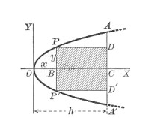
\includegraphics[height=3cm,width=3cm]{parabola-pblm.eps}
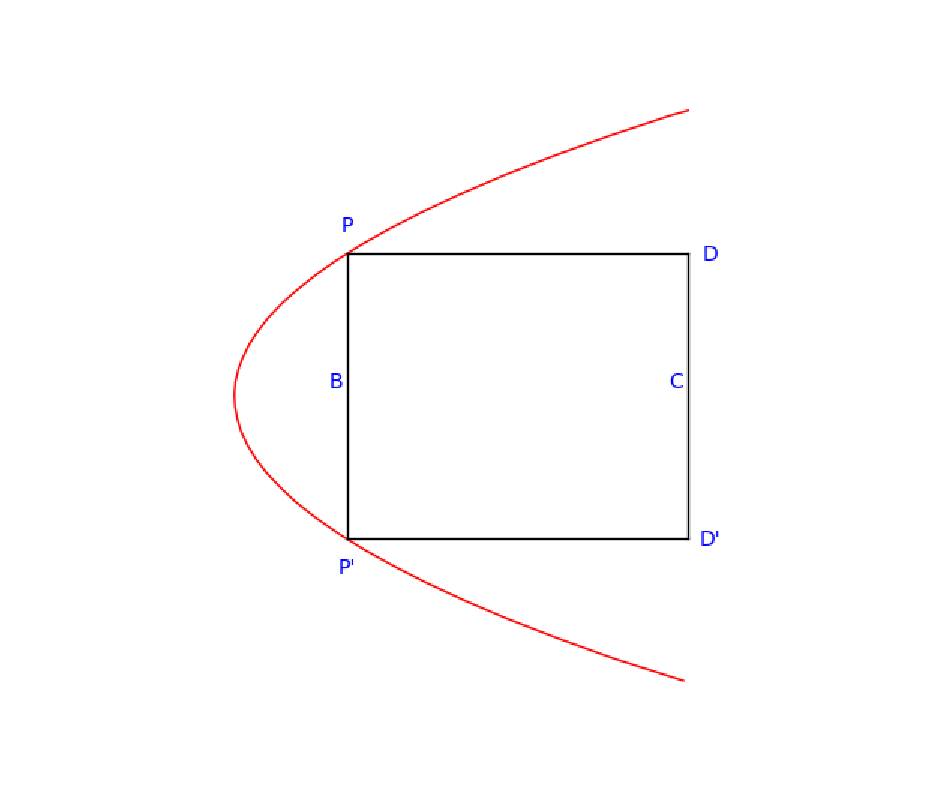
\includegraphics[height=6cm,width=9cm]{parabola-pblm3.eps}
\end{center}
\end{minipage}
%\caption{Scan of Granville's graphic of an inscribed rectangle in a parabola.}
\caption{An inscribed rectangle in a parabola, $P=(x,y)$.}
\label{fig:parabola-pblm}
\end{figure}

HINT. If $OC = h$, $BC = h - x$ and $PP' = 2y$; therefore the 
area of rectangle $PDD'P'$ is $2(h - x)y$.

But since P lies on the parabola $y^2 = 2px$, the function to be tested is
$2(h - x)\sqrt{2px}$

Ans. Width = $\frac{2}{3} h$.

\item
%4
Find the altitude of the cone of maximum volume that can be 
inscribed in a sphere of radius $r$ (see Figure \ref{fig:cone-pblm}).

\begin{figure}[h!]
%\begin{tabular}{cc}
\begin{minipage}{\textwidth}
\begin{center}
%\vspace{1.0 cm}
%\includegraphics[height=3cm,width=3cm]{cone-pblm.eps}
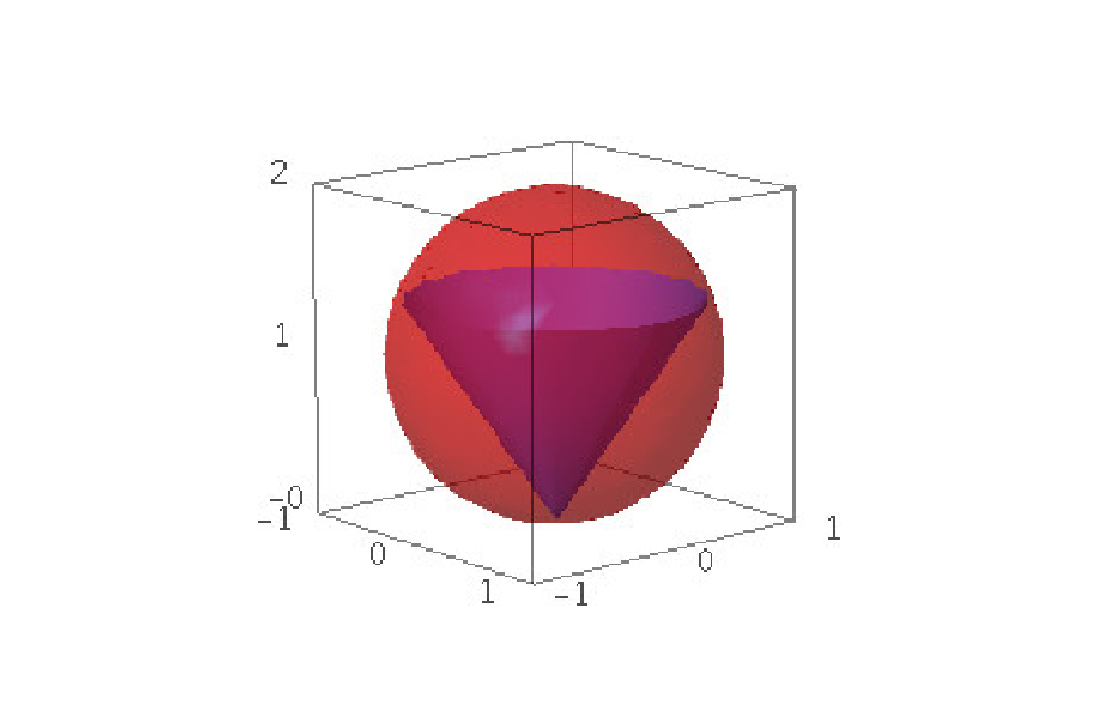
\includegraphics[height=6cm,width=9cm]{cone-pblm3.eps}
\end{center}
\end{minipage}
%\caption{Scan of Granville's graphic of an inscribed cone in a sphere.}
\caption{An inscribed cone, height $y$ and base radius $x$, in a sphere.} 
\label{fig:cone-pblm}
\end{figure}
%sage: p1 = parametric_plot3d([cos(u)*v, sin(u)*v, 3*v/2-1/3], (u, 0, 2*pi), (v, 0, 0.95),plot_points=[20,20])
%sage: p2 = sphere((0,0,2/3), color='red', opacity=0.5, aspect_ratio=[1,1,1])
%sage: show(p1+p2)

HINT. Volume of cone = $\frac{1}{3} \pi x^2 y$. But $x^2= BC \times CD = y(2r - y)$; 
therefore the function to be tested is
$ f(y) = \frac{\pi}{3} y^2 (2r - y)$.

Ans. Altitude of cone = $\frac{4}{3}r$.

\item
%5
Find the altitude of the cylinder of maximum volume that can be inscribed 
in a given right cone  (see Figure \ref{fig:cone-pblm2}).

\begin{figure}[h!]
%\begin{tabular}{cc}
\begin{minipage}{\textwidth}
\begin{center}
%\vspace{1.0 cm}
%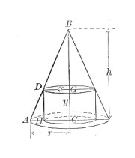
\includegraphics[height=3cm,width=3cm]{cone-pblm2.eps}
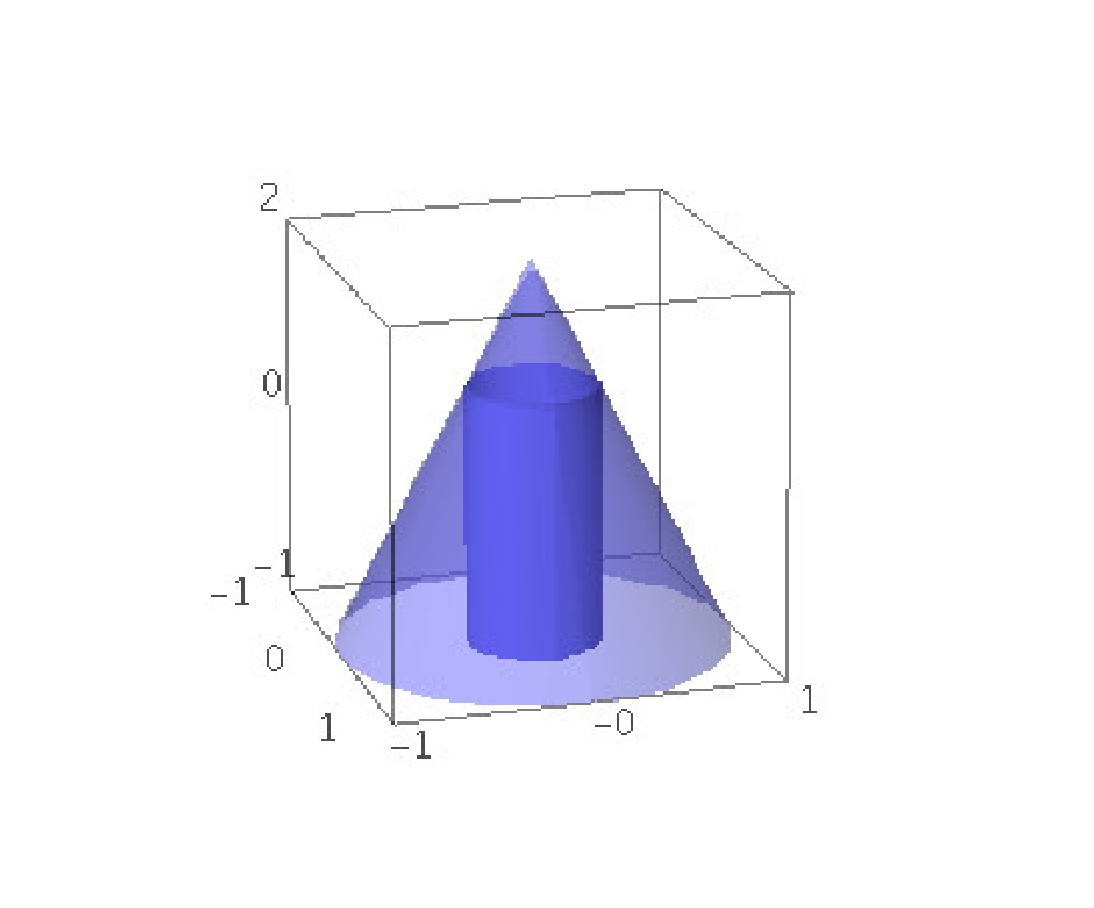
\includegraphics[height=6cm,width=6cm]{cone-pblm4.eps}
\end{center}
\end{minipage}
%\caption{Scan of Granville's graphic of an inscribed cylinder in a cone.}
\caption{An inscribed cylinder in a cone.}
\label{fig:cone-pblm2}
\end{figure}
%sage: p1 = parametric_plot3d([cos(u)*v, sin(u)*v, 3/2-3*v/2], (u, 0, 2*pi), (v, 0, 1.5), opacity = 0.5, plot_points=[20,20])
%sage: p2 = parametric_plot3d([cos(u)/2, sin(u)/2, v-3/4], (u, 0, 2*pi), (v, 0, 3/2), plot_points=[20,20])
%sage: show(p1+p2)

\noindent
HINT. Let $AU = r$ and $BC = h$. Volume of cylinder = $\pi x^2y$. 
But from similar triangles ABC and DBG,
$r/x =h/(h-y)$, so $x = \frac{r(h - y)}{h}$.
Hence the function to be tested is
$ f(y) = \frac{r^2}{h^2} y(h - y)^2$.

\noindent
Ans. Altitude = $\frac{1}{3}h$.

\item
%6
Divide $a$ into two parts such that their product is a maximum.

Ans. Each part $= \frac{a}{2}$.

\item
%7
Divide $10$ into two such parts that the sum of the double of one and 
square of the other may be a minimum.

Ans. $9$ and $1$.

\item
%8
Find the number that exceeds its square by the greatest possible quantity.

Ans. $\frac{1}{2}$.

\item
%9
What number added to its reciprocal gives the least possible sum?

Ans. $1$.

\item
%10
Assuming that the stiffness of a beam of rectangular cross 
section varies directly as the breadth and the cube of the depth, 
what must be the breadth of the stiffest beam that can be cut from 
a log $16$ inches in diameter?

Ans. Breadth $= 8$ inches.

\item
%11
A water tank is to be constructed with a square base and open top, 
and is to hold $64$ cubic yards. If the cost of the sides is \$ 1 a 
square yard, and of the bottom \$ 2 a square yard, what are the 
dimensions when the cost is a minimum? What is the minimum cost?

Ans. Side of base = $4$ yd., height = $4$ yd., cost \$ 96.

\item
%12
A rectangular tract of land is to be bought for the purpose of 
laying out a quarter-mile track with straightaway sides and 
semicircular ends. In addition a strip $35$ yards wide along each 
straightaway is to be bought for grand stands, training quarters, 
etc. If the land costs \$ 200 an acre, what will be the maximum 
cost of the land required? 

Ans. \$ 856.

\item
%13
A torpedo boat is anchored $9$ miles from the nearest point 
of a beach, and it is desired to send a messenger in the shortest 
possible time to a military camp situated $15$ miles from that 
point along the shore. If he can walk $5$ miles an hour but row 
only $4$ miles an hour, required the place he must land.

Ans. $3$ miles from the camp.

\item
%14
A gas holder is a cylindrical vessel closed at the top and 
open at the bottom, where it sinks into the water. What should be 
its proportions for a given volume to require the least material 
(this would also give least weight)?

Ans. Diameter = double the height.

\item
%15
What should be the dimensions and weight of a gas holder of 
$8,000,000$ cubic feet capacity, built in the most 
economical manner out of sheet iron $\frac{1}{16}$ of an inch 
thick and weighing $\frac{5}{2}$ lb. per sq. ft.?

Ans. Height = $137$ ft., diameter = $273$ ft., weight = $220$ tons.

\item
%16
A sheet of paper is to contain $18$ sq. in. of printed matter. 
The margins at the top and bottom are to be $2$ inches each and 
at the sides $1$ inch each. Determine the dimensions of the 
sheet which will require the least amount of paper.

Ans. $5$ in. by $10$ in.

\item
%17
A paper-box manufacturer has in stock a quantity of 
strawboard $30$ inches by $14$ inches. Out of this material he 
wishes to make open-top boxes by cutting equal squares out of each 
corner and then folding up to form the sides. Find the side of 
the square that should be cut out in order to give the 
boxes maximum volume.

Ans. $3$ inches.

\item
%18
A roofer wishes to make an open gutter of maximum capacity whose 
bottom and sides are each $4$ inches wide and whose sides have the 
same slope. What should be the width across the top?

Ans. $8$ inches. $4$

\item
%19
Assuming that the energy expended in driving a steamboat through 
the water varies as the cube of her velocity, find her most economical 
rate per hour when steaming against a current running $c$ miles per hour.

HINT. Let 	$v$ 	= most economical speed;
then 	$av^3$ 	= energy expended each hour, $a$ being a 
constant depending upon the particular conditions,
and 	$v - c$	= actual distance advanced per hour.
Hence $\frac{av^3}{v - c}$ is the energy expended per mile of 
distance advanced, and it is therefore the function whose minimum is wanted.

\item
%20
Prove that a conical tent of a given capacity will require 
the least amount of canvas when the height is $\sqrt{2}$ times the 
radius of the base. Show that when the canvas is laid out flat it 
will be a circle with a sector of $152^0 9'= 2.6555... $ cut out. 
A bell tent $10$ ft. high should then have a base of diameter $14$ ft. 
and would require $272$ sq. ft. of canvas.

\item
%21
A cylindrical steam boiler is to be constructed having a capacity of 
$1000$ cu. ft. The material for the side costs \$ 2 a square foot, 
and for the ends \$ 3 a square foot. Find radius when the cost is the least.

Ans. $\frac{1}{\sqrt[3]{3\pi}}$ ft.

\item
%22
In the corner of a field bounded by two perpendicular roads a spring 
is situated $6$ rods from one road and $8$ rods from the other. 

(a) How should a straight road be run by this spring and across the 
corner so as to cut off as little of the field as possible?

(b) What would be the length of the shortest road that could be run across?

Ans. (a) $12$ and $16$ rods from corner.
(b) $(6^{\frac{2}{3}} + 8^{\frac{2}{3}})^{\frac{3}{2}}$ rods.

\item
%23
Show that a square is the rectangle of maximum perimeter that can be 
inscribed in a given circle.

\item
%24
Two poles of height a and b feet are standing upright and are $c$ feet apart. 
Find the point on the line joining their bases such that the sum 
of the squares of the distances from this point to the tops of the poles is a minimum.
(Ans. Midway between the poles.)
When will the sum of these distances be a minimum?

\item
%25
A conical tank with open top is to be built to contain $V$ cubic feet. 
Determine the shape if the material used is a minimum.

\item
%26
An isosceles triangle has a base $12$ in. long and altitude $10$ in. 
Find the rectangle of maximum area that can be inscribed 
in it, one side of the rectangle coinciding with the base of the triangle.

\item
%27
Divide the number $4$ into two such parts that the sum of the 
cube of one part and three times the square of the other shall have a maximum value.

\item
%28
Divide the number $a$ into two parts such that the product of 
one part by the fourth power of the other part shall be a maximum.

\item
%29
A can buoy in the form of a double cone is to be made from two equal 
circular iron plates of radius $r$. Find the radius of the base of the cone 
when the buoy has the greatest displacement (maximum volume).

Ans. $r \sqrt{\frac{2}{3}}$.

\item
%30
Into a full conical wineglass of depth $a$ and generating angle $a$ 
there is carefully dropped a sphere of such size as to cause the 
greatest overflow. Show that the radius of the sphere is
$\frac{\alpha \sin \alpha}{\sin \alpha \cos 2 \alpha}$.

\item
%31
A wall $27$ ft. high is $8$ ft. from a house. Find the length of the 
shortest ladder that will reach the house if one end rests on the 
ground outside of the wall.

Ans. $13 \sqrt{13}$.

Here's how to solve this using \sage:
Let $h$ be the height above ground at which the ladder hits the 
house and let $d$ be the distance from the wall that the ladder 
hits the ground on the other side of the wall. By similar triangles,
$h/27=(8+d)/d=1+\frac{8}{d}$, so $d+8 = 8\frac{h}{h-27}$. 
The length of the ladder is,
by the Pythagorean theorem, 
$f(h) = \sqrt{h^2+(8+d)^2}=\sqrt{h^2+(8\frac{h}{h-27})^2}$.

\vskip .1in

{\small{
\begin{Verbatim}[fontsize=\small,fontfamily=courier,fontshape=tt,frame=single,label=\sage]

sage: h = var("h")
sage: f(h) = sqrt(h^2+(8*h/(h-27))^2)
sage: f1(h) = diff(f(h),h)
sage: f2(h) = diff(f(h),h,2)
sage: crit_pts = solve(f1(h) == 0,h); crit_pts
[h == 21 - 6*sqrt(3)*I, h == 6*sqrt(3)*I + 21, h == 39, h == 0]
sage: h0 = crit_pts[2].rhs(); h0
39
sage: f(h0)
13*sqrt(13)
sage: f2(h0)
3/(4*sqrt(13))

\end{Verbatim}
}}
\vskip .1in

\noindent
This says $f(h)$ has four critical points, but only one of which is 
meaningful, $h_0=39$. At this point, $f(h)$ is a minimum.

\item
%32
A vessel is anchored $3$ miles offshore, and opposite a point $5$ 
miles further along the shore another vessel is anchored $9$ miles 
from the shore. A boat from the first vessel is to land a passenger 
on the shore and then proceed to the other vessel.
What is the shortest course of the boat?

Ans. $13$ miles.

\item
%33
A steel girder $25$ ft. long is moved on rollers along a passageway 
$12.8$ ft. wide and into a corridor at right angles to the passageway. 
Neglecting the width of the girder, how wide must the corridor be?

Ans. $5.4$ ft.

\item
%34
A miner wishes to dig a tunnel from a point A to a point B $300$ 
feet below and $500$ feet to the east of A. Below the level of A 
it is bed rock and above A is soft earth. If the cost of tunneling 
through earth is \$ 1 and through rock \$ 3 per linear foot, 
find the minimum cost of a tunnel.

Ans. \$ 1348.53.

\item
%35
A carpenter has $108$ sq. ft. of lumber with which to build a box with 
a square base and open top. Find the dimensions of the largest 
possible box he can make.

Ans. $6 \times 6 \times 3$.

\item
%36
Find the right triangle of maximum area that can be constructed on a 
line of length $h$ as hypotenuse.

Ans. $\frac{h}{\sqrt{2}}$ = length of both legs.

\item
%37
What is the isosceles triangle of maximum area that can be inscribed 
in a given circle?

Ans. An equilateral triangle.

\item
%38
Find the altitude of the maximum rectangle that can be inscribed 
in a right triangle with base $b$ and altitude $h$.

Ans. Altitude = $\frac{h}{2}$.

\item
%39
Find the dimensions of the rectangle of maximum area that can be inscribed 
in the ellipse $b^2x^2 + a^2y^2 = a^2b^2$.

Ans. $a \sqrt{2}\times b \sqrt{2}$; area = $2ab$.

\item
%40
Find the altitude of the right cylinder of maximum volume that 
can be inscribed in a sphere of radius $r$.

Ans. Altitude of cylinder = $\frac{2r}{\sqrt{3}}$.

\item
%41
Find the altitude of the right cylinder of maximum convex (curved) 
surface that can be inscribed in a given sphere.

Ans. Altitude of cylinder = $r \sqrt{2}$.

\item
%42
What are the dimensions of the right hexagonal prism of minimum 
surface whose volume is $36$ cubic feet?

Ans. Altitude = $2 \sqrt{3}$; side of hexagon = $2$.

\item
%43
Find the altitude of the right cone of minimum volume circumscribed 
about a given sphere.

Ans. Altitude = $4r$, and volume = $2\times$ vol. of sphere.

\item
%44
A right cone of maximum volume is inscribed in a given right cone, 
the vertex of the inside cone being at the center of the base of 
the given cone. Show that the altitude of the inside cone is one 
third the altitude of the given cone.

\item
%45
Given a point on the axis of the parabola $y^2 = 2px$ at a distance 
$a$ from the vertex; find the abscissa of the point of the curve nearest to it.

Ans. $x = a - p$.

\item
%46
What is the length of the shortest line that can be drawn 
tangent to the ellipse $b^2x^2 + a^2y^2 = a^2b^2$ and 
meeting the coordinate axes?

Ans. $a + b$.

\item
%47
A Norman window consists of a rectangle surmounted by a 
semicircle. Given the perimeter, required the height and 
breadth of the window when the quantity of light admitted is a maximum.

Ans. Radius of circle = height of rectangle.

\item
%48
A tapestry $7$ feet in height is hung on a wall so that its lower 
edge is $9$ feet above an observer's eye. At what distance from the 
wall should he stand in order to obtain the most favorable view?
(HINT. The vertical angle subtended by the tapestry in the eye of the 
observer must be at a maximum.)

Ans. $12$ feet.

\item
%49
What are the most economical proportions of a tin can which shall have 
a given capacity, making allowance for waste?
(HINT. There is no waste in cutting out tin for the side of the can, but 
for top and bottom a hexagon of tin circumscribing the circular pieces 
required is used up.
%\noindent
NOTE 1. If no allowance is made for waste, then height = diameter.
%\noindent
NOTE 2. We know that the shape of a bee cell is hexagonal, giving a 
certain capacity for honey with the greatest possible economy of wax.)

Ans. Height = $\frac{2 \sqrt{3}}{\pi} \times$ diameter of base.

\item
%50
An open cylindrical trough is constructed by bending a given sheet of 
tin at breadth $2a$. Find the radius of the cylinder of which the 
trough forms a part when the capacity of the trough is a maximum.

Ans. Rad. = $\frac{2a}{\pi}$; i.e. it must be bent in the form of a semicircle.

\item
%51
A weight $W$ is to be raised by means of a lever with the force $F$ 
at one end and the point of support at the other. If the weight is 
suspended from a point at a distance $a$ from the point of support, 
and the weight of the beam is $w$ pounds per linear foot, what 
should be the length of the lever in order that the force required 
to lift it shall be a minimum?

Ans. $x = \sqrt{\frac{2aW}{w}}$ feet.

\item
%52
An electric arc light is to be placed directly over the center of a 
circular plot of grass $100$ feet in diameter. Assuming that the 
intensity of light varies directly as the sine of the angle under 
which it strikes an illuminated surface, and inversely as the square 
of its distance from the surface, how high should the light he 
hung in order that the best possible light shall fall on a walk along 
the circumference of the plot?

Ans. $\frac{50}{\sqrt{2}}$ feet

\item
%53
The lower corner of a leaf, whose width is $a$, is folded over so as just 
to reach the inner edge of the page. 

\begin{figure}[h!]
%\begin{tabular}{cc}
\begin{minipage}{\textwidth}
\begin{center}
%\vspace{1.0 cm}
%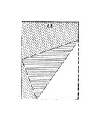
\includegraphics[height=3cm,width=2cm]{leaf.eps}
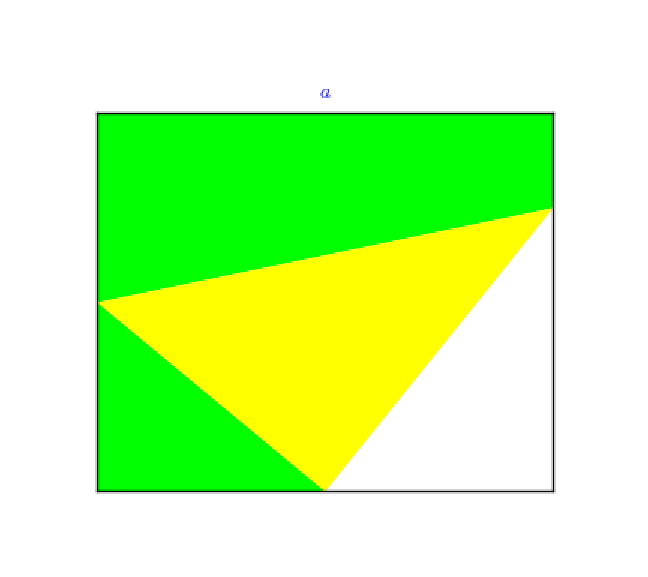
\includegraphics[height=5cm,width=3cm]{leaf2.eps}
\end{center}
\end{minipage}
%\caption{Scan of Granville's graphic of a leafed page.}
\caption{A leafed page of width $a$.}
\label{fig:leaf}
\end{figure}

(a) Find the width of the part folded over when the length of the 
crease is a minimum. 

(b) Find the width when the area folded over is a minimum.

Ans. (a) $\frac{3}{4}a$; (b) $\frac{2}{3}a$.

\item
%54
A rectangular stockade is to be built which must have a certain 
area. If a stone wall already constructed is available for one of 
the sides, find the dimensions which would make the cost of construction the least.

Ans. Side parallel to wall = twice the length of each end.

%\item
%%55
%A cow is tethered by a perfectly smooth rope, a slip noose in the rope 
%being thrown over a large square post. If the cow pulls the rope 
%taut in the direction shown in the figure, at what angle will the 
%rope leave the post?
%
%\begin{figure}[h!]
%%\begin{tabular}{cc}
%\begin{minipage}{\textwidth}
%\begin{center}
%%\vspace{1.0 cm}
%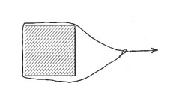
\includegraphics[height=2cm,width=4cm]{tether.eps}
%\end{center}
%\end{minipage}
%\caption{Scan of Granville's graphic of a tethered post.}
%\label{fig:tether}
%\end{figure}
%
%Ans. $30^o$.

\item
%56
When the resistance of air is taken into account, the inclination 
of a pendulum to the vertical may be given by the formula
$\theta= ae^{-kt}\cos\, (nt + \eta)$.
Show that the greatest elongations occur at equal intervals 
$\frac{\pi}{n}$ of time.

\item
%57
 It is required to measure a certain unknown magnitude $x$ with precision. 
Suppose that $n$ equally careful observations of the magnitude 
are made, giving the results
$ a_1, a_2, a_3, \dots, a_n$.
The errors of these observations are evidently
$ x - a_1, x - a_2, x - a_3, \cdots, x - a_n$,
some of which are positive and some negative.
It has been agreed that the most probable value of $x$ is such that it 
renders the sum of the squares of the errors, namely
$(x - a_1)^2 + (x - a_2)^2 + (x - a_3)^2 + \cdots + (x - a_n)^2$,
a minimum. Show that this gives the arithmetical mean of the 
observations as the most probable value of $x$.

(This is related to the method of least squares, discovered by Gauss,
a commonly used technique in statistical applications.) %% new

\item
%58
The bending moment at $x$ of a beam of length $\ell$, uniformly loaded, 
is given by the formula
$  M = \frac{1}{2} w\ell x - \frac{1}{2} wx^2$,
where $w$ = load per unit length. Show that the maximum bending 
moment is at the center of the beam.

\item
%59
 If the total waste per mile in an electric conductor is
$  W = c^2 r + \frac{t^2}{r}$, 
where $c$ = current in amperes (a constant), 
$r$ = resistance in ohms per mile, and 
$t$ = a constant depending on the interest on the investment 
and the depreciation of the plant, what is the relation 
between $c$, $r$, and $t$ when the waste is a minimum?

Ans. $cr = t$.

\item
%60
A submarine telegraph cable consists of a core of copper wires 
with a covering made of nonconducting material. If x denote the ratio 
of the radius of the core to the thickness of the covering, it is known 
that the speed of signaling varies as

\[
    x^2 \log \frac{1}{x}.
\]
Show that the greatest speed is attained when $x = \frac{1}{\sqrt{e}}$.

\item
%61
Assuming that the power given out by a voltaic cell is given by the formula

\[
    P = \frac{E^2 R}{(r + R)^2},
\]
when $E$ = constant electromotive force, 
$r$ = constant internal resistance, 
$R$ = external resistance, prove that $P$ is a maximum when $r = R$.

\item
%62
The force exerted by a circular electric current of radius $a$ on a small 
magnet whose axis coincides with the axis of the circle varies as

\[
    \frac{x}{(a^2 + x^2)^{\frac{5}{2}}}.
\]
where $x$ = distance of magnet from plane of circle. Prove that the 
force is a maximum when $x = \frac{a}{2}$.

\item
%63
We have two sources of heat at A and B, which we visualize on the
real line (with B to the right or A), with intensities $a$ and $b$ respectively. 
%
%\begin{figure}[h!]
%%\begin{tabular}{cc}
%\begin{minipage}{\textwidth}
%\begin{center}
%%\vspace{1.0 cm}
%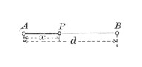
\includegraphics[height=1.5cm,width=7cm]{heat-sources.eps}
%\end{center}
%\end{minipage}
%\caption{Scan of Granville's graphic of two heat sources.}
%\label{fig:heat-sources}
%\end{figure}
%
%\noindent
The total intensity of heat at a point P between A and B at a distance of $x$ from A 
is given by the formula
$I = \frac{a}{x^2} + \frac{b}{(d - x)^2}$.
Show that the temperature at P will be the lowest when
$    \frac{d - x}{x} = \frac{\sqrt[3]{b}}{\sqrt[3]{a}}$.
that is, the distances BP and AP have the same ratio as the cube roots 
of the corresponding heat intensities. The distance of P from A is
$x = \frac{a^{\frac{1}{3}} d}{a^{\frac{1}{3}} + b^{\frac{1}{3}} }$.
 
\item
%64
The range of a projectile in a vacuum is given by the formula
$ R = \frac{v_0^2 \sin 2\phi}{g}$,
where $v_0$ = initial velocity, $g$ = acceleration due to gravity, 
$\phi$ = angle of projection with the horizontal. 
Find the angle of projection which gives the greatest range for a 
given initial velocity.

Ans. $\phi  = 45^o=\pi/4$.

\item
%65
The total time of flight of the projectile in the last problem is given by the formula
$   T = \frac{2v_0 \sin \phi}{g}$.
At what angle should it be projected in order to make the time of flight a maximum?

Ans. $\phi  = 90^o=\pi/2$.

\item
%66
The time it takes a ball to roll down an inclined plane with angle
$\phi$ (with respect to the $x$-axis) is given by the formula
$ T = 2\sqrt{\frac{2}{g \sin 2\phi}}$.
Neglecting friction, etc., what must be the value of $\phi$ to 
make the quickest descent?

Ans. $\phi  = 45^o=\pi/4$.

\item
%67
Examine the function $(x - 1)^2(x + 1)^3$ for maximum and minimum 
values. Use the first method.

Solution. $f(x) = (x - 1)^2(x + 1)^3$.

First step. $f'(x) = 2(x - 1)(x + 1)^3 + 3(x - 1)^2(x + 1)^2 
= (x - 1)(x + 1)^2(5x - 1)$.

Second step. $(x - 1)(x + 1)^2(5x - 1)= 0$,
$x = 1, -1, \frac{1}{5}$, which are critical values.

Third step. $f'(x) = 5(x -1) (x + 1)^2 (x - \frac{1}{5})$.

Fourth step. 	Examine first for critical value $x = 1$.

When $x < 1$, $f'(x) = 5( - )( + )2( + ) = -$.
When $x > 1$, $f'(x) = 5( + )( + )2( + ) = +$.
Therefore, when $x = 1$ the function has a minimum value 
$f(l) = 0$.
Examine now for the critical value $x = \frac{1}{5}$.
When $x < \frac{1}{5}$, $f'(x) = 5(-) (+)^2 (-) = +$.
When $x > \frac{1}{5}$, $f'(x) = 5(-) (+)^2 (+) = -$.
Therefore, when $x = \frac{1}{5}$ the function has a maximum value 
$f(\frac{1}{5}) = 1.11$.
Examine lastly for the critical value $x = -1$.
When $x < - 1$, $f'(x) = 5( - )( - )2( - ) = +$.
When $x > - 1$, $f'(x) = 5( - )( + )2( - ) = +$.
Therefore, when $x = - 1$ the function has neither a maximum nor a minimum value.

\item
%68

\end{enumerate}

Examine the following functions for maximum and minimum values:

\begin{enumerate}
\addtocounter{enumi}{68}
\item
%69
$(x - 3)^2(x - 2)$. 	

Ans. 	$x = \frac{7}{3}$, gives max. = $\frac{4}{27}$;
$x = 3$, gives min. = $0$.

\item
%70
$(x - 1)^3(x - 2)^2$. 

Ans. $x = \frac{8}{5}$, gives max. = $0.03456$;
$x = 2$, gives min. = $0$; $x = 1$, gives neither.

\item
%71
$(x - 4)^5(x + 2)^4$. 	

Ans. $x = - 2$, gives max.;
$x = \frac{2}{3}$ gives min; $x = 4$, gives neither.

\item
%72
$(x - 2)^5(2x + 1)^4$. 

Ans. $x = -\frac{1}{2}$, gives max.;
  $x = \frac{11}{18}$, gives min.;
  	$x = 2$, gives neither.

\item
%73
$(x + 1)^{\frac{2}{3}}(x - 5)^2$.

\begin{figure}[h!]
%\begin{tabular}{cc}
\begin{minipage}{\textwidth}
\begin{center}
%\vspace{1.0 cm}
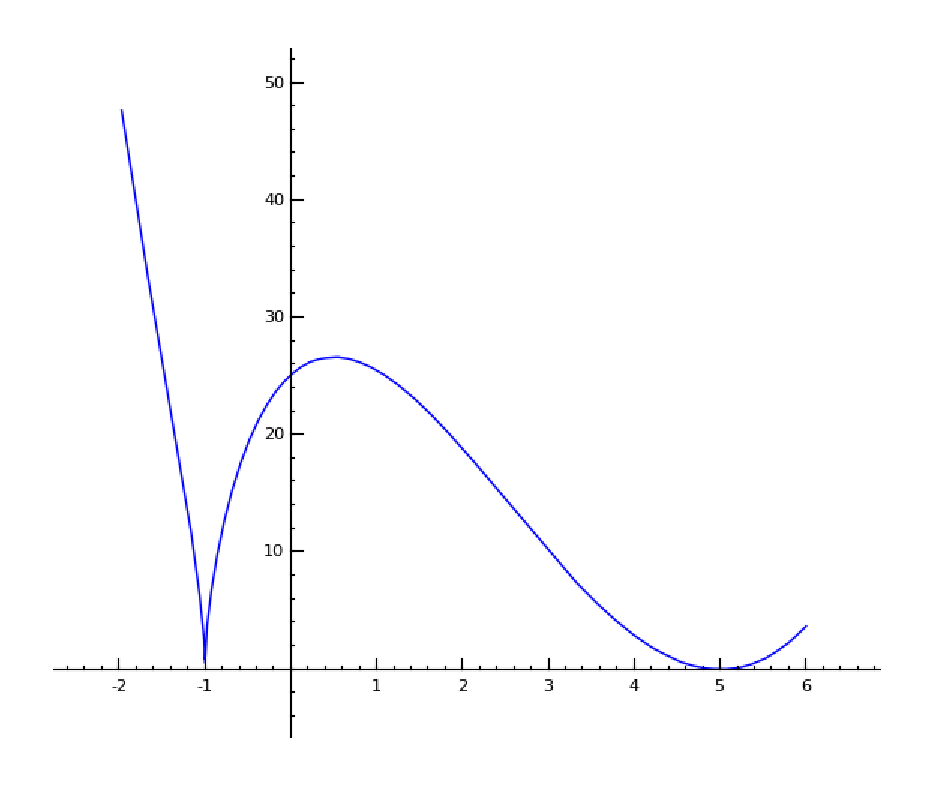
\includegraphics[height=3cm,width=5cm]{ch8-prblm73.eps}
\end{center}
\end{minipage}
\caption{\sage plot of $y=(x + 1)^{\frac{2}{3}}(x - 5)^2$.}
\label{fig:ch8-prblm73}
\end{figure}
%sage: P = plot(((x + 1)^2)^(1/3)*(x - 5)^2,-2,6)
%sage: show(P)

Ans. $ 	x = \frac{1}{2}$, gives max.;
 $x = -1$ and $5$, give min.

\item
%74
$(2x - a)^{\frac{1}{3}} (x - a)^{\frac{2}{3}}$. 

Ans. $	x = \frac{2a}{3}$, gives max.;
  	$x = 1$ and $-\frac{1}{3}$, gives min.;
  	$x = \frac{a}{2}$, gives neither.

\item
%75
$x(x - 1)^2(x + 1)^3$.

Ans. $x = \frac{1}{2}$, gives max.;
$x = 1$ and $-\frac{1}{3}$, gives min.;
$x = -1$, gives neither.

\item
%76
$x(a + x)^2(a - x)^3$ 	

Ans. $x = -a$ and $\frac{a}{3}$, give max.;
  	$x = -\frac{a}{2}$;
  	$x = a$, gives neither.

\item
%77
$b + c(x - a)^{\frac{2}{3}}$.

Ans. $x = a$, gives min. = $b$.

\item
%78
$a - b(x - c)^{\frac{1}{3}}$. 

Ans. No max. or min.

\item
%79
$\frac{x^2 - 7x + 6}{x - 10}$.

Ans. $x = 4$, gives max.
  $x = 16$, gives min.

\item
%80
$\frac{(a - x)^3}{a - 2x}$.

Ans. $x = \frac{a}{4}$, gives min.

\item
%81
$\frac{1 - x + x^2}{1 + x - x^2}$.

Ans. $	x = \frac{1}{2}$, gives min.

\item
%82
$\frac{x^2 - 3x + 2}{x^2 + 3x +2}$.

Ans. $x = \sqrt{2}$, gives min. = $12\sqrt{2} - 17$;
$x = -\sqrt{2}$, gives max. = $-12\sqrt{2} - 17$;
$x = - 1, - 2$, give neither.

\item
%83
$\frac{(x - a)(b - x)}{x^2}$.

$x = \frac{2ab}{a + b}$, gives max. = $\frac{(a - b)^2}{4ab}$.

\item
%84
$\frac{a^2}{x} + \frac{b^2}{a - x}$.

Ans. $x = \frac{a^2}{a - b}$, gives min.;
$x = \frac{a^2}{a + b}$, gives max.

\item
%85
Examine $x^3 - 3x^2 - 9x + 5$ for maxima and minima, 
Use the second method, \S \ref{sec:84}. %, p.113.

Solution. $f(x) 	= x^3 - 3x^2 - 9x + 5$.

First step. 	$f'(x) 	= 3x^2 - 6x - 9$.

Second step, 	$3x^2 - 6x - 9 	= 0$;
hence the critical values are $x = -1$ and $3$.

Third step. 	$f''(x) 	= 6x - 6$.

Fourth step. $f''(-1) 	= -12$.

Therefore, $f(-1) 	= 10 =$  maximum value.
$f''(3) = + 12$. Therefore, $f(3) = - 22 =$ minimum value.

\item
%86
Examine $\sin^2x\cos\, x$ for maximum and minimum values.

Solution. $f(x) = \sin^2x\cos\, x$.

First step. $f'(x) = 2\sin\, x\cos^2x - \sin^3x$.

Second step. $2\sin\, x\cos^2x - \sin^3x = 0$;
hence the critical values are $x = n\pi$
and $x = n\pi \pm \arctan( -\sqrt{2}) = n\pi \pm \alpha$.

Third step. 	$f''(x) = \cos\, x(2\cos^2x - 7\sin^2x)$.

Fourth step. $f''(0) = +$. Therefore,	$f(0)=0$ = minimum value.
  	$f''(\pi) 	= -$. Therefore,$f(\pi) = 0$ = maximum value.
  	$f''(\alpha) 	= -$. Therefore, $f(\alpha)$ maximum value.
  	$f''(\pi - \alpha)= +$. Therefore,$f(\pi - \alpha)$ minimum value.

\end{enumerate}

Examine the following functions for maximum and minimum values:

\begin{enumerate}
\addtocounter{enumi}{86}

\item
%87
$3x^3 - 9x^2 - 27x + 30$. 	

Ans. 	$x = -1$, gives max. = $45$;
  	$x = 3$, gives min. = $- 51$.

\item
%88
$2x^3 - 21x^2 + 36x - 20$. 

Ans. $x = 1$, gives max. = $-3$;
$x = 6$, gives min. = $-128$.

\item
%89
$\frac{x^3}{3} - 21x^2 + 3x + 1$. 

Ans. $x = 1$, gives max. = $\frac{7}{3}$;
$x = 3$, gives min. = $1$.

\item
%90
$2x^3 - 15x^2 + 36x + 10$.

Ans. $x = 2$, gives max. = $38$;
$x = 3$, gives min. = $37$.

\item
%91
$x^3 - 9x^2 + 15x - 3$. 

Ans. $x = 1$, gives max. = $4$;
$x = 5$, gives min. = $- 28$.

\item
%92
$x^3 - 3x^2 + 6x + 10$.

Ans.  	No max. or min.

\item
%93
$x^5 - 5x^4 + 5x^3 + 1$. $x = 1$, gives max. = $2$;
$x = 3$, gives min. = $-26$; $x = 0$, gives neither.

\item
%94
$3x^5 - 125x^2 + 2160x$. 

$x = -4$ and $3$, give max.;
$x = -3$ and $4$, give min.

\item
%95
$2x^3 - 3x^2 - 12x + 4$.

\item
%96
$2x^3 - 21x^2 + 36x - 20$.

\item
%97
$x^4 - 2x^2 + 10$.

\item
%98
$x^4 - 4$.

\item
%99
$x^3 - 8$.

\item
%100
$4 - x^6$.

\item
%101
$\sin\,x(1 + \cos\,x)$. 	

Ans. 	$x = 2n\pi + \frac{\pi}{3}$, give max. $= \frac{3}{4}\sqrt{3}$;
  	$x = 2n\pi - \frac{\pi}{3}$, give min. $= \frac{3}{4}\sqrt{3}$;
  	$x = n\pi$, give neither.

\item
%102
$\frac{x}{\log x}$.

Ans. $	x = e$, gives min. = $e$;
$x = 1$, gives neither.

\item
%103
$\log\, \cos\, x$.

Ans. $	x = n\pi$, gives max.

\item
%104
$ae^{kx} + be^{- kx}$.

Ans. $ 	x = \frac{1}{k} \log \sqrt{\frac{b}{a}}$, gives min. $= 2\sqrt{ab}$.

\item
%105
$x^x$. 	  
	
$x = \frac{1}{e}$, gives min.

\item
%106
$x^{\frac{1}{x}}$.

Ans. $x = e$, gives max.

\item
%107
$\cos\, x + \sin\, x$. 

Ans. $x = \frac{\pi}{4}$, gives max. = $\sqrt{2}$.
$x = \frac{5\pi}{4}$, gives min. = $-\sqrt{2}$.

\item
%108
$\sin\, 2x - x$.

Ans. $ 	x = \frac{\pi}{6}$, gives max.;
$x = -\frac{\pi}{6}$, gives min.

\item
%109
$x + \tan\, x$.

Ans. 	No max. or min.

\item
%110
$\sin^3x\cos\, x$. 

Ans. $x = n \pi + \frac{\pi}{3}$, gives max. = $\frac{3}{16} \sqrt{3}$;
$x = n \pi - \frac{\pi}{3}$, gives min. = $-\frac{3}{16} \sqrt{3}$;
$x = n\pi$, gives neither.

\item
%111
$x \ \cos\, x$. 	

\begin{figure}[h!]
%\begin{tabular}{cc}
\begin{minipage}{\textwidth}
\begin{center}
%\vspace{1.0 cm}
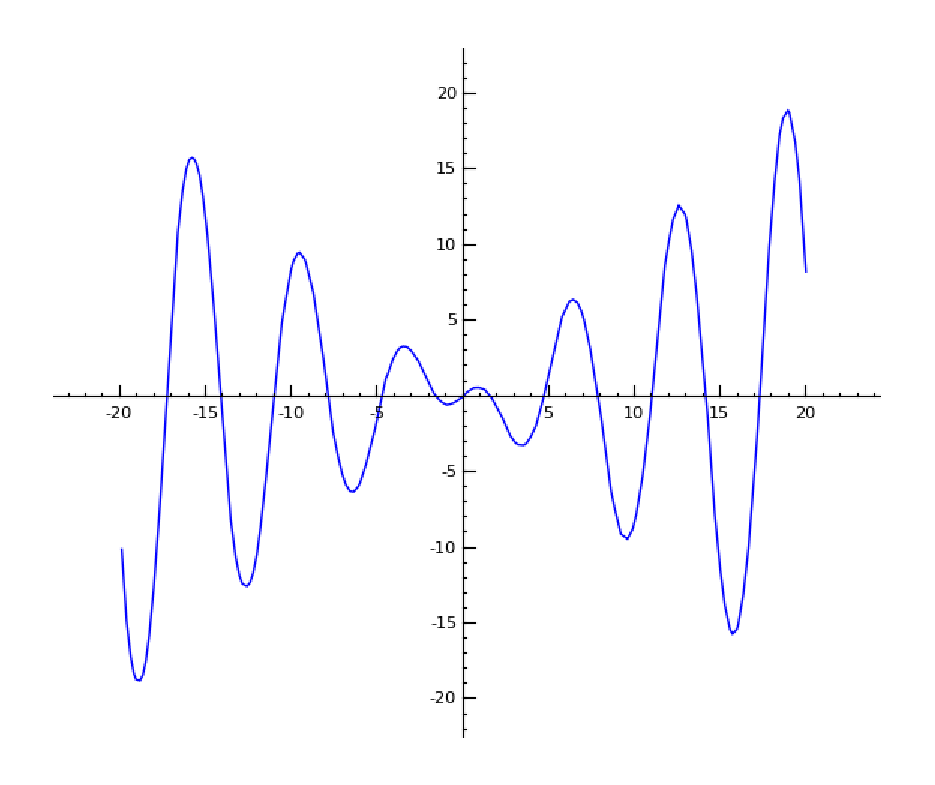
\includegraphics[height=3cm,width=5cm]{ch8-prblm111.eps}
\end{center}
\end{minipage}
\caption{\sage plot of $y=x\cos(x)$.}
\label{fig:ch8-prblm11}
\end{figure}
%sage: P = plot(x*cos(x),-20,20)
%sage: show(P)

Ans. $x$ such that $x\sin\, x = \cos\, x$, gives max/min. 
%% typo in text??

\item
%112
$\sin\,x + \cos\, 2x$. 

Ans. $\arcsin \frac{1}{4}$, gives max.;
 $x = \frac{\pi}{2}$, gives min.

\item
%113
$2\tan\, x - \tan^2x$.

Ans. $ 	x = \frac{\pi}{4}$, gives max.

\item
%114
$\frac{\sin x}{1 + \tan x}$. 

Ans. $	x = \frac{\pi}{4}$, gives max.

\item
%115
$\frac{x}{1 + x \tan x}$. 

$x = \cos\, x$, gives max.;
$x = -\cos\, x$, gives min.

\end{enumerate}


%85. 
\section{Points of inflection}
\label{sec:85}

\begin{definition}
{\rm 
{\it Points of inflection} separate arcs concave upwards from arcs 
concave downwards. They may also be defined as points where

(a) $\frac{d^2 y}{dx^2} = 0$ and $\frac{d^2 y}{dx^2}$ changes sign,

\noindent
or 

(b) $\frac{d^2 x}{dy^2} = 0$ and $\frac{d^2 x}{dy^2}$ changes sign.
}
\end{definition}

Thus, if a curve $y = f(x)$ changes from concave upwards to concave 
downwards at a point, or the reverse, then such a point 
is called a {\it point of inflection}.
\index{point of inflection}

From the discussion of \S \ref{sec:84}, %§84 
it follows at once that where the curve is concave up, $f''(x) = +$, 
and where the curve is concave down, $f''(x) = -$. 
In order to change sign it must pass through the value 
zero\footnote{It is assumed that $f'(x)$ and $f''(x)$ are 
continuous. The solution of Exercise 2, \S \ref{sec:85}, %p. 127 [§85], 
shows how to discuss a case where $f'(x)$ and $f''(x)$ are both infinite.};
%Evidently salient points (see \S \ref{sec:156}) %p. 258 [§156]) 
%are excluded, since at such points $f'(x)$ is discontinuous.};
hence we have:

%  (23) 
\begin{lemma}
\label{lemma:85-23}
{\rm At points of inflection, $f''(x) = 0$}. 
\end{lemma}

Solving the equation resulting from Lemma \ref{lemma:85-23}
gives the abscissas of the points of inflection. To determine the 
direction of curving or direction of bending in the vicinity of a 
point of inflection, test $f''(x)$ for values of $x$, first a trifle 
less and then a trifle greater than the abscissa at that point.

If $f''(x)$ changes sign, we have a point of inflection, and the 
signs obtained determine if the curve is concave upwards or concave 
downwards in the neighborhood of each point of inflection.

The student should observe that near a point where the curve 
is concave upwards the curve lies above the tangent, and at a 
point where the curve is concave downwards the curve lies below the 
tangent. At a point of inflection the tangent evidently crosses the curve.

Following is a {\it rule for finding points of inflection} of 
the curve whose equation is $y = f(x)$. This rule includes also 
directions for examining the direction of curvature of the curve 
in the neighborhood of each point of inflection.

\begin{itemize}
\item
FIRST STEP. Find $f''(x)$.

\item
SECOND STEP. Set $f''(x) = 0$, and solve the resulting equation for real roots.

\item
THIRD STEP. Write $f''(x)$ in factor form.

\item
FOURTH STEP. Test $f''(x)$ for values of $x$, first a trifle less and 
then a trifle greater than each root found in the second step. 
If $f''(x)$ changes sign, we have a point of inflection.
\end{itemize}

When $f''(x) = +$, the curve is concave upwards\footnote{This may be 
easily remembered if we say that a vessel shaped like the curve 
where it is concave upwards will hold ($+$) water, and where it is 
concave downwards will spill ($-$) water.}.

When $f''(x) = -$, the curve is concave downwards.

\section{Examples}

Examine the following curves for points of inflection and direction 
of bending.

\begin{enumerate}

\item
%1
 $y = 3x^4 - 4x^3 + 1$.

Solution. $f(x) = 3x^4 - 4x^3 + 1$.

First step. $f''(x) 	= 36x^2 - 24x$.

Second step. $36x^2 - 24x 	= 0$,
$x = \frac{2}{3}$ and $x = 0$, critical values.

Third step. $f''(x) = 36x(x - \frac{2}{3})$.

Fourth step. 	When $x < 0$, $f''(x) = +$; and when 
$x > 0$, $f''(x) = -$. Therefore, the curve is concave upwards 
to the left and concave downwards to the right of $x = 0$. % (A in figure).
When $x < \frac{2}{3}$, $f''(x) = -$; and when $x > \frac{2}{3}$, $f''(x) = +$.
Therefore, the curve is concave downwards to the left and 
concave upwards to the right of $x = \frac{2}{3}$. % (B in figure).

The curve is evidently concave upwards everywhere to the 
left of $x=0$, concave downwards between $(0,1)$ and 
$(\frac{2}{3}, \frac{11}{27})$, and concave upwards everywhere to the 
right of $(\frac{2}{3}, \frac{11}{27})$.

\item
%2
$(y - 2)^3 = (x - 4)$.

Solution. $y 	= 2 + (x - 4)^{-\frac{1}{3}}$.

First step. $\frac{dy}{dx} 	= \frac{1}{3}(x - 4)^{-\frac{2}{3}}$.

Second step. 	When $x = 4$, both first and second derivatives are infinite.

Third step. 	When $x < 4$, $\frac{d^2 y}{dx^2} = +$; but when 
$x > 4$, $\frac{d^2 y}{dx^2} = -$.

We may therefore conclude that the tangent at $(4, 2)$ is 
perpendicular to the $x$-axis, that to the left of $(4,2)$ the curve 
is concave upwards, and to the right of $(4, 2)$ it is concave downwards. 
Therefore $(4, 2)$ must be considered a point of inflection.

\item
%3
$y = x^2$. 	

Ans. 	Concave upwards everywhere.

\item
%4
$y = 5 - 2x - x^2$. 

Ans.  	Concave downwards everywhere.

\item
%5
$y = x^3$. 	  	

Ans. Concave downwards to the left and concave upwards to the right of $(0, 0)$.

\item
%6
$y = x^3 - 3x^2 - 9x + 9$. 

Ans.  	Concave downwards to the left and concave upwards to the right of $(1, -2)$.

\item
%7
$y = a + (x - b)^3$. 	  	

Ans. Concave downwards to the left and concave upwards to the right of $(b, a)$.

\item
%8
$a^2 y = \frac{x^3}{3} - a x^2 + 2 a^3$.

Ans. Concave downwards to the left and concave upwards to 
the right of $(a, \frac{4a}{3})$.

\item
%9
$y = x^4$. 	  	

Ans. Concave upwards everywhere.

\item
%10
$y = x^4 - 12x^3 + 48x^2 - 50$. 	

Ans. Concave upwards to the left of $x = 2$, concave downwards 
between $x = 2$ and $x = 4$, concave upwards to the right of $x = 4$.

\item
%11
$y = \sin\, x$. 

Ans. 	Points of inflection are $x = n\pi$, $n$ being any integer.

\item
%12
$y = \tan\,x$. 	

Ans. 	Points of inflection are x = nπ, n being any integer.

\item
%13
Show that no conic section can have a point of inflection.

\item
%14
Show that the graphs of $e^x$ and $\log\, x$ have no points of inflection.

\end{enumerate}

%86. 
\section{Curve tracing}

The elementary method of tracing (or plotting) a curve whose 
equation is given in rectangular coordinates, and one with which 
the student is already familiar, is to solve its equation for $y$ (or $x$), 
assume arbitrary values of $x$ (or $y$), calculate the corresponding 
values of $y$ (or $x$), plot the respective points, and draw 
a smooth curve through them, the result being an approximation 
to the required curve. This process is laborious at best, and 
in case the equation of the curve is of a degree higher than 
the second, the solved form of such an equation may be unsuitable 
for the purpose of computation, or else it may fail altogether, 
since it is not always possible to solve the equation for $y$ or $x$.

The general form of a curve is usually all that is desired, and the 
Calculus furnishes us with powerful methods for determining 
the shape of a curve with very little computation.

The first derivative gives us the slope of the curve at any 
point; the second derivative determines the intervals within 
which the curve is concave upward or concave downward, and the 
points of inflection separate these intervals; the maximum points 
are the high points and the minimum points are the low points 
on the curve. As a guide in his work the student may follow the

Rule for tracing curves. Rectangular coordinates.

\begin{itemize}
\item
FIRST STEP. 
Find the first derivative; place it equal to zero; solving gives 
the abscissas of maximum and minimum points.

\item
SECOND STEP. Find the second derivative; place it equal to zero; 
solving gives the abscissas of the points of inflection.

\item
THIRD STEP. Calculate the corresponding ordinates of the 
points whose abscissas were found in the first two steps. 
Calculate as many more points as may be necessary to give a 
good idea of the shape of the curve. Fill out a table such as 
is shown in the example worked out.

\item
FOURTH STEP. Plot the points determined and sketch in the curve 
to correspond with the results shown in the table.
\end{itemize}

If the calculated values of the ordinates are large, it is 
best to reduce the scale on the $y$-axis so that the general 
behavior of the curve will be shown within the limits of the 
paper used. Coordinate plotting (graph) paper should be employed.

\section{Exercises}

Trace the following curves, making use of the above rule. 
Also find the equations of the tangent and normal at each point of inflection.

\begin{enumerate}

\item
%1
$y = x^3 - 9x^2 + 24x - 7$.

Solution. Use the above rule.

First step. $y' = 3x^2 - 18x + 24$,
$3x^2 - 18x + 24 	= 0$, $	x 	= 2,4$.

Second step. $y'' 	= 6x - 18$, $6x - 18 	= 0$,
$x 	= 3$.

Third step.

\begin{tabular}{cccccc}
$x$ &	$y$ &	$y'$ &	$y''$& 	Remarks &	Direction of Curve\\
0 &	-7& 	+ &	- &	        &     concave down   \\
2 &	13 &	0 &	- &       max.  &     concave down         \\
3 &	11 &	- &	0  &   pt. of infl. & concave up  \\
4 &	9 &	0 &	+ &    min. 	&   concave up     \\
6 &	29 &	+ &	+ &            &  concave up \

\end{tabular}

Fourth step. Plot the points and sketch the curve. %, we get the figure shown. 
To find the equations of the tangent 
and normal to the curve at the point of inflection $(3,11)$, use 
formulas (\ref{eqn:1-65}), ((\ref{eqn:65-2}). %, pp. 76, 77 [§65]. 
This gives $3x + y = 20$ for the tangent and $3y - x = 30$ for the normal.

\item
%2
$y = x^3 - 6x^2 - 36x + 5$.

Ans. Max. $(-2, 45)$; min. $(6, -211)$; pt. of infl. $(2, -83)$; 
tan. $y + 48x - 13 = 0$; nor. $48y - x + 3986 = 0$.

We shall solve this using \sage.

\vskip .1in

\begin{Verbatim}[fontsize=\small,fontfamily=courier,fontshape=tt,frame=single,label=\sage]

sage: x = var("x")
sage: f = x^3 - 6*x^2 - 36*x + 5
sage: f1 = diff(f(x),x); f1
3*x^2 - 12*x - 36
sage: crit_pts = solve(f1(x) == 0, x); crit_pts
[x == 6, x == -2]
sage: f2 = diff(f(x),x,2); f2(x)
6*x - 12
sage: x0 = crit_pts[0].rhs(); x0
6
sage: x1 = crit_pts[1].rhs(); x1
-2
sage: f(x0); f2(x0)
-211
24
sage: f(x1); f2(x1)
45
-24
sage: infl_pts = solve(f2(x) == 0, x); infl_pts
[x == 2]
sage: p = plot(f, -5, 10)
sage: show(p)

\end{Verbatim}
\vskip .1in

\noindent


\begin{figure}[h!]
%\begin{tabular}{cc}
\begin{minipage}{\textwidth}
\begin{center}
%\vspace{1.0 cm}
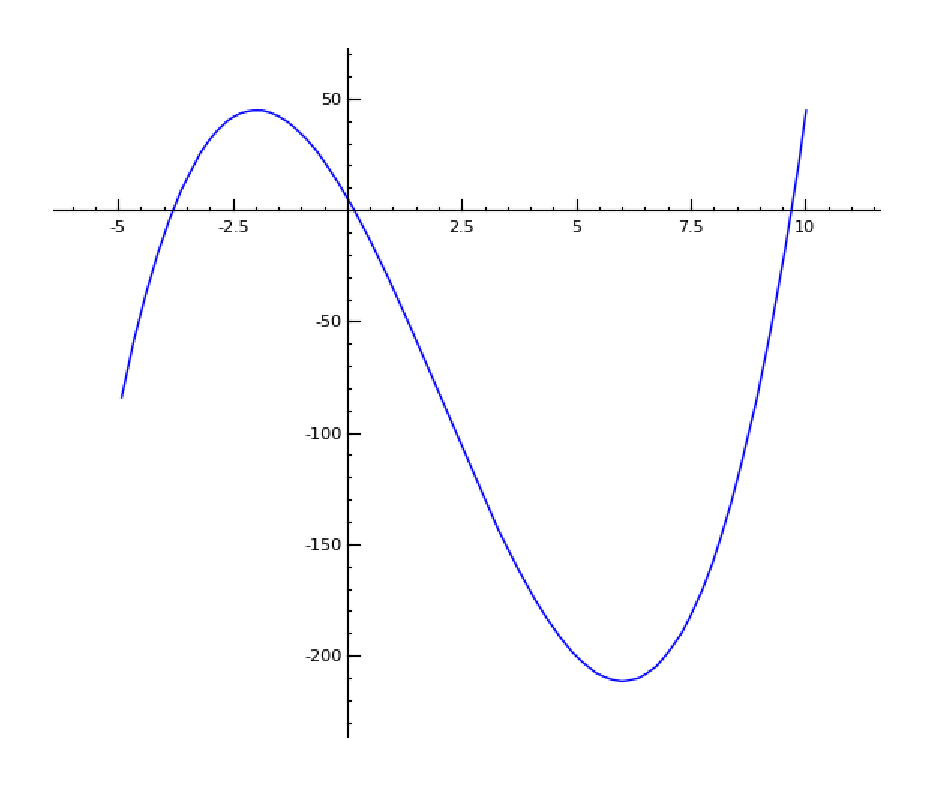
\includegraphics[height=5cm,width=7cm]{exercise-8-11-2.eps}
\end{center}
\end{minipage}
\caption{Plot for Exercise 8.11-2, $y=x^3 - 6x^2 - 36x + 5$.}
\label{fig:exercise-8-11-2}
\end{figure}


\item
%3
$y = x^4 - 2x^2 + 10$.

Ans. Max. $(0, 10)$; min. $(\pm 1, 9)$; pt. of infl. 
$\left ( \pm \frac{1}{\sqrt{3}}, \frac{85}{9} \right )$.

\item
%4
$y = \frac{1}{2}x^4 - 3x^2 + 2$.

Ans. Max. $(0, 2)$; min. $(\pm \sqrt{3}, -\frac{5}{2} )$; 
pt. of infl. $(\pm 1, -\frac{1}{2})$.

\item
%5
$y = \frac{6x}{1 + x^2}$.

Ans. Max. $(1, 3)$; min. $(-1, -3)$; pt. of infl. $(0, 0)$, 
$\left ( \pm \sqrt{3}, \pm \frac{3\sqrt{3}}{2} \right )$.

\item
%6
$y = 12x - x^3$.

Ans. Max. $(2, 16)$; min. $(-2, -16)$; pt. of infl. $(0, 0)$.

\item
%7
$4y + x^3 - 3x^2 + 4 = 0$.

Ans. Max. $(2,0)$; min. $(0, -1)$.

\item
%8
$y = x^3 - 3x^2 - 9x + 9$.

\item
%9
$2y + x^3 - 9x + 6 = 0$.

\item
%10
$y = x^3 - 6x^2 - 15x + 2$.

\item
%11
$y(1 + x^2) = x$.

\item
%12
$y = \frac{8a^3}{x^2 + 4a^2}$.

\item
%13
$y = e^{-x^2}$.

\item
%14
$y = \frac{4 + x}{x^2}$.

\item
%15
$y = (x + l)^{\frac{2}{3}}(x - 5)^2$.

\item
%16
$y = \frac{x + 2}{x^3}$.

\item
%17
$y = x^3 - 3x^2 - 24x$.

\item
%18
$y = 18 + 36x - 3x^2 - 2x^3$.

\item
%19
$y = x - 2\cos\, x$.

\item
%20
$y = 3x - x^3$.

\item
%21
$y = x^3 - 9x^2 + 15x - 3$.

\item
%22
$x^2y = 4 + x$.

\item
%23
$4y = x^4 - 6x^2 + 5$.

\item
%24
$y = \frac{x^3}{x^2 + 3a^2}$.

\item
%25
$y = \sin\, x + \frac{x}{2}$.

\item
%26
$y = \frac{x^2 + 4}{x}$.

\item
%27
$y = 5x - 2x^2 - \frac{1}{3}x^3$.

\item
%28
$y = \frac{1 + x^2}{2x}$.

\item
%29
$y = x - 2\sin\, x$.

\item
%30
$y = \log\, \cos\, x$.

\item
%31
$y = \log(1 + x^2)$.

\end{enumerate}
